\documentclass[10pt]{article}


\usepackage{latexsym}
\usepackage{amsmath}
\usepackage{amssymb}
\usepackage{amsfonts}
\usepackage{amsthm}
\usepackage{amscd}
\usepackage{epsfig}
\usepackage{verbatim}
\usepackage{fancybox}
\usepackage{moreverb}
\usepackage{graphicx}
\usepackage{psfrag}
\usepackage{hyperref}
\usepackage[all]{xy}
\usepackage[toc,page]{appendix}
\usepackage[subnum]{cases}
\usepackage{bm}
\usepackage{framed}
\usepackage{color}
\usepackage{dsfont}
\usepackage{textcomp}
\usepackage{graphicx}
\usepackage{url}

\textheight 22cm    \textwidth 16cm
\voffset=-1cm
\hoffset=-1.2cm


\newcommand{\C}{{\mathbb C}}
\newcommand{\R}{{\mathbb R}}
\newcommand{\N}{{\mathbb N}}
\newcommand{\Z}{{\mathbb Z}}
\newcommand{\Q}{{\mathbb Q}}
\newcommand{\T}{{\mathbb T}}
\newcommand{\E}{{\mathbb E}}
\newcommand{\di}{{\mathbb D}}
\newcommand{\Y}{{\mathbf Y}}
\newcommand{\D}{{\partial}}
\newcommand{\Cl}{{\mathcal C}}
\newcommand{\Pa}{{\mathcal P}}
\newcommand{\Flux}{{\mathcal F}}
\newcommand{\B}{{\mathfrak B}}
\newcommand{\M}{{\mathcal M}}
\newcommand{\dis}{{\mathcal D}}
\newcommand{\A}{{\mathcal{A}}}
\newcommand{\fin}{\rule{1ex}{1ex}}


\newtheorem{theorem}{Theorem}
\newtheorem{lemma}[theorem]{Lemma}
\newtheorem{proposition}[theorem]{Proposition}
\newtheorem{corollary}[theorem]{Corollary}
\newtheorem{definition}[theorem]{Definition}
\newtheorem{example}[theorem]{Example}
\newtheorem{remark}[theorem]{Remark}
\newtheorem{notation}[theorem]{Notation}
\newtheorem{hypothesis}[theorem]{Hypothesis}


\renewcommand{\thesection}{\arabic{section}}
\renewcommand{\thelemma}{\thesection\arabic{lemma}}
\renewcommand{\theproposition}{\thesection\arabic{proposition}}
\renewcommand{\thetheorem}{\thesection\arabic{theorem}}
\renewcommand{\thecorollary}{\thesection\arabic{corollary}}
\renewcommand{\thedefinition}{\thesection\arabic{definition}}
\renewcommand{\theexample}{\thesection\arabic{example}}
\renewcommand{\theremark}{\thesection\arabic{remark}}
\renewcommand{\thenotation}{\thesection\arabic{notation}}
\renewcommand{\theequation}{\thesection.\arabic{equation}}
\def\commutatif{\ar@{}[rd]|{\circlearrowleft}}


\title{\textbf{\underline{Report :} Numerical simulation of charged particle beams in an electro-magnetic focusing field}}


\author{Alexandre Temperville, Master 2 Scientific Computing}

\date{01/08/2012}





\begin{document}

\maketitle

\newpage

\tableofcontents \clearpage




\section{First part : Modelization}


\subsection{Question 1.1.}


We want to reduce the six following equations with some hypotheses : \\

\begin{subnumcases}{\label{VM3D}}
\cfrac{\D f}{\D t} + \mathbf{v} \cdot \nabla_{\mathbf{x}} f + \cfrac{q}{\gamma_{z}\,m}\, ( \mathbf{E} + \mathbf{v} \times \mathbf{B}) \cdot \nabla_{\mathbf{v}}f = 0 \, , & \textnormal{(Vlasov)} \label{Vlasov3D} \\
f(t=0,\mathbf{x},\mathbf{v}) = f^{0}(\mathbf{x},\mathbf{v}) \, , & \textnormal{(initial data)} \label{initial3D} \\
\cfrac{\D \mathbf{B}}{\D t} + \nabla_{\mathbf{x}} \times \mathbf{E} = 0 \, , & \textnormal{(Faraday)} \label{Faraday3D} \\
\cfrac{1}{c^{2}}\,\cfrac{\D \mathbf{E}}{\D t} + \mu_{0}\,\mathbf{J} = \nabla_{\mathbf{x}} \times \mathbf{B} \, , & \textnormal{(Amp\`ere)} \label{Ampere3D} \\
\nabla_{\mathbf{x}} \cdot \mathbf{E} = \cfrac{\rho}{\varepsilon_{0}} \, , & \textnormal{(Gauss)} \label{Gauss3D} \\
\nabla_{\mathbf{x}} \cdot \mathbf{B} = 0 \, , & \textnormal{(Maxwell)} \label{Thomson3D}
\end{subnumcases} \\

We have the four following hypotheses : \\

\begin{itemize}
\item[(i)] The beam has reached its stationary state,
\item[(ii)] The particles propagate at a constant longitudinal velocity $v_{z}$,
\item[(iii)] The longitudinal parts of the self-consistent electric and magnetic fields are neglected,
\item[(iv)] The space domain in the $z$-direction is of the form $[0,L_{z}]$, $z = 0$ corresponding to the source of the beam. \\
\end{itemize}

That means : \\

\begin{itemize}
\item[(i)] $\frac{\D f}{\D t} = 0$, $\frac{\D \mathbf{B}}{\D t} = \frac{\D \mathbf{E}}{\D t} = \mathbf{0}$, $\frac{\D \mathbf{B^{e}}}{\D t} = \frac{\D \mathbf{E^{e}}}{\D t} = \mathbf{0}$, $\frac{\D \mathbf{B^{s}}}{\D t} = \frac{\D \mathbf{E^{s}}}{\D t} = \mathbf{0}$.

\item[(ii)] $v_{z} = constant \Rightarrow \nabla_{\mathbf{v}}f = \left( \begin{array}{c}
E_{x}^{e} + v_{y}\,B_{z}^{e} - v_{z}\,B_{y}^{e} \\
E_{y}^{e} + v_{z}\,B_{x}^{e} - v_{x}\,B_{z}^{e}
\end{array} \right)$.
\item[(iii)] We can consider these two vectors in 2D as their third component is supposed to be 0 :

$\mathbf{E^s} = \left( \begin{array}{c}
E_x^s \\
E_y^s \\
0
\end{array} \right) \sim \left( \begin{array}{c}
E_x^s \\
E_y^s
\end{array} \right)$ and
$\mathbf{B^s} = \left( \begin{array}{c}
B_x^s \\
B_y^s \\
0
\end{array} \right) \sim \left( \begin{array}{c}
B_x^s \\
B_y^s
\end{array} \right) $.


\item[(iv)] The space domain in the $z$-direction is of the form $[0,L_{z}]$, $z = 0$ corresponding to the source of the beam. \\
\end{itemize}


\subsubsection{Relation (1.4d)}


With the Faraday Equation (1.1c), we have : \\
$\nabla_{\mathbf{x}} \times \mathbf{E} = - \frac{\D \mathbf{B}}{\D t} = \mathbf{0}$
then
$\nabla_{\mathbf{x}} \times \mathbf{E^s} = - \frac{\D \mathbf{B^s}}{\D t} = \mathbf{0}$ so \\

$$\boxed{\exists \phi^{s} \text{ such that } \mathbf{E^s} = - \nabla_{\mathbf{x}}\phi^{s}}$$ \\


\subsubsection{Relation (1.4e)}


With the Gauss Equation (1.1e), we have : \\
$\nabla_{\mathbf{x}} \cdot \mathbf{E^s} = \nabla_{\mathbf{x}} \cdot \left( - \nabla_{\mathbf{x}}\phi^{s} \right) = \cfrac{\rho}{\varepsilon_{0}}$

hence $- \Delta_{\mathbf{x}} \phi^{s} = \frac{\rho}{\varepsilon_{0}} = \frac{q}{\varepsilon_{0}}.\int_{\mathbb{R}^3} f(t,\mathbf{x},\mathbf{v}).\delta_{\{v_z\}}.d\mathbf{v}$ so \\
$$\boxed{- \Delta_{\mathbf{x}} \phi^{s} = \frac{q}{\varepsilon_{0}}.\int_{\mathbb{R}^2} f(t,\mathbf{x},\mathbf{v}).d\mathbf{v}} $$ \\


\subsubsection{Relation (1.4b)}


With the initial data (1.1b), at $t = 0$, we are on $z = 0$, $v_z$ is constant so we can consider that : \\
$f(t=0,x,y,z,v_x,v_y,v_z) = f(z=0,x,y,v_x,v_y)$.

We define $f_p^0(\mathbf{x},\mathbf{v}) = f^0(x,y,0,v_x,v_y,v_z)$ and we get : \\
$$\boxed{f(z=0,\mathbf{x},\mathbf{v}) = f_p^0(\mathbf{x},\mathbf{v})}$$ \\



\subsubsection{Relations (1.4a) and (1.4c)}


With the Vlasov equation (1.1a), we have :

$$ 0 = \underbrace{\frac{\D f}{\D t}}_{=0} + \mathbf{v} \cdot \nabla_{\mathbf{x}}f + \frac{q}{\gamma_{z}\,m}\,(\mathbf{E}+\mathbf{v}\times\mathbf{B}) \cdot \nabla_{\mathbf{v}}f : (*)$$

Let us compute $\mathbf{E}+\mathbf{v}\times\mathbf{B}$ :
\begin{align*}
\mathbf{E}+\mathbf{v}\times\mathbf{B} &= \mathbf{E^e} + \mathbf{E^s} +
\left( \begin{array}{c}
v_x \\
v_y \\
v_z
\end{array} \right) \times
\left( \begin{array}{c}
B_x^e + B_x^s \\
B_y^e + B_y^s \\
B_z^e
\end{array} \right) \\
&= \mathbf{E^e} + \mathbf{E^s} +
\left( \begin{array}{c}
v_y\,B_z^e - v_z\,B_y^e - v_z\,B_y^s \\
v_z\,B_x^e + v_z\,B_x^s - v_x\,B_z^e \\
v_x\,B_y^e + v_x\,B_y^s - v_y\,B_x^e - v_y\,B_x^s
\end{array} \right) \\
&= \mathbf{E^e} +
\left( \begin{array}{c}
v_y\,B_z^e - v_z\,B_y^e \\
v_z\,B_x^e - v_x\,B_z^e \\
v_x\,B_y^e - v_y\,B_x^e
\end{array} \right)
+ \mathbf{E^s} + 
\left( \begin{array}{c}
- v_z\,B_y^s \\
v_z\,B_x^s \\
v_x\,B_y^s - v_y\,B_x^s
\end{array} \right) 
\end{align*}

We define 
$\mathbf{F}^{e} = \cfrac{q}{v_{z}\,\gamma_{z}\,m}\, \left(
\begin{array}{c}
E_{x}^{e} + v_{y}\,B_{z}^{e} - v_{z}\,B_{y}^{e} \\
E_{y}^{e} + v_{z}\,B_{x}^{e} - v_{x}\,B_{z}^{e} \\
E_{z}^{e} + v_{x}\,B_{y}^{e} - v_{y}\,B_{x}^{e}
\end{array}
\right)$ so we have :

$$
\cfrac{q}{v_{z}\,\gamma_{z}\,m}\,(\mathbf{E}+\mathbf{v}\times\mathbf{B}) = \mathbf{F}^{e} + \cfrac{q}{v_{z}\,\gamma_{z}\,m}\,\mathbf{E^s} + \cfrac{q}{v_{z}\,\gamma_{z}\,m}\,\mathbf{v} \times \mathbf{B^s}
$$

As we have to multiply $\mathbf{E}+\mathbf{v}\times\mathbf{B}$ by $\nabla_{\mathbf{v}}f$ and that the third component of $\nabla_{\mathbf{v}}f$ is 0, we can consider that :
$$\boxed{\mathbf{F}^{e} \sim \cfrac{q}{v_{z}\,\gamma_{z}\,m}\, \left(
\begin{array}{c}
E_{x}^{e} + v_{y}\,B_{z}^{e} - v_{z}\,B_{y}^{e} \\
E_{y}^{e} + v_{z}\,B_{x}^{e} - v_{x}\,B_{z}^{e}
\end{array}
\right)}$$


With the new notations in 2D, the relation (*) becomes :
$$ 0 = \underbrace{v_x\,\frac{\D f}{\D x} + v_y\,\frac{\D f}{\D y}}_{=\mathbf{v} \cdot  \nabla_{\mathbf{x}}f} + v_z\,\frac{\D f}{\D z} + v_z\,\mathbf{F}^{e} \cdot \nabla_{\mathbf{v}}f + \frac{q}{\gamma_{z}\,m}\,(\mathbf{E^s}+\mathbf{v}\times\mathbf{B^s}) \cdot \nabla_{\mathbf{v}}f : (*)$$

Then, we can divide this relation by $v_z$ and modify this relation thanks to the previous calculations :
$$ 0 = \frac{\D f}{\D z} + \frac{\mathbf{v}}{v_z} \cdot \nabla_{\mathbf{x}}f + \mathbf{F}^{e} \cdot \nabla_{\mathbf{v}}f + \frac{q}{v_z\,\gamma_{z}\,m}\,(\mathbf{E^s}+\mathbf{v}\times\mathbf{B^s}) \cdot \nabla_{\mathbf{v}}f : (*)$$

Let us try to simplify the last term of this equation. With the Maxwell equation (1.1f), we have :\\

$\mathbf{B^s} = (B_x^s;B_y^s;0)$ is such that $\nabla_{\mathbf{x}} \cdot \mathbf{B^s} = 0$ so $\exists \psi^{s}:\mathbb{R}^3\rightarrow\mathbb{R}$ such that $\mathbf{B^s} = \left(\frac{\D \psi^{s}}{\D y}; - \frac{\D \psi^{s}}{\D x};0\right)$. \\

$$\mathbf{v} \times \mathbf{B^s} = \left( \begin{array}{c}
v_x \\
v_y \\
v_z
\end{array} \right) \times \left(
\begin{array}{c}
\frac{\D \psi^{s}}{\D y} \\
- \frac{\D \psi^{s}}{\D x}\\
0
\end{array} \right) = \left( \begin{array}{c}
v_z\,\frac{\D \psi^{s}}{\D x} \\
v_z\,\frac{\D \psi^{s}}{\D y} \\
- v_x\,\frac{\D \psi^{s}}{\D x} - v_y\,\frac{\D \psi^{s}}{\D y}
\end{array} \right) \sim v_z\,\nabla_{\mathbf{x}}\psi^s$$ (as we will multiply this with a vector which has its third component equal to 0, we can neglect now the third component). \\

With the Ampere equation (1.1d), we have : \\
$$\mu_{0}\,\mathbf{J} = \nabla_{\mathbf{x}} \times \mathbf{B} = \left( \begin{array}{c}
\frac{\D}{\D x} \\
\frac{\D}{\D y} \\
\frac{\D}{\D z}
\end{array} \right) \times \left(
\begin{array}{c}
\frac{\D \psi^{s}}{\D y} \\
- \frac{\D \psi^{s}}{\D x}\\
0
\end{array} \right) = \left( \begin{array}{c}
\frac{\D^2}{\D z \D x}\psi^{s} \\
\frac{\D^2}{\D z \D y}\psi^{s} \\
- \frac{\D^2}{\D x^2}\psi^{s} - \frac{\D^2}{\D y^2}\psi^{s}
\end{array} \right)$$

Let us expand the three components of \textbf{J} (we consider that $\frac{\D^2 \psi^s}{\D z^2}$ is negligible) and with the previous equality we have :


\begin{displaymath}
  \left\lbrace
     \begin{array}{ll}
\mu_{0}\,q\,\int_{\mathbb{R}^3} v_x\,f\,d\mathbf{v} = \frac{\D^2}{\D z \D x}\psi^{s} \\
\mu_{0}\,q\,\int_{\mathbb{R}^3} v_y\,f\,d\mathbf{v} = \frac{\D^2}{\D z \D y}\psi^{s} \\
v_z\,\mu_{0}\,\underbrace{q\,\int_{\mathbb{R}^3} f\,d\mathbf{v}}_{\rho} = - \Delta_{\mathbf{x}} \psi^{s}
    \end{array}
  \right.
\end{displaymath} 

With the Gauss equation, we can modify the third equation in:

$$\underbrace{\mu_{0}\,\epsilon_{0}}_{\frac{1}{c^2}}\,v_z\,\nabla_{\mathbf{x}} \cdot \mathbf{E^s} = - \Delta_{\mathbf{x}} \psi^{s}$$
Using the following relation : $\frac{v_z}{c^2} = \frac{1}{v_z}\,\frac{v_z^2}{c^2} = \frac{1}{v_z}\,\left(1 - \frac{1}{\gamma_{z}^{2}}\right)$ and the relation (1.4d) found previously, we obtain : \\
$$\frac{1}{v_z}\,\left(1 - \frac{1}{\gamma_{z}^{2}}\right).\left(- \Delta_{\mathbf{x}} \phi^{s}\right) = - \Delta_{\mathbf{x}} \psi^{s}$$
So, if we choose $\psi^{s}$ as the following, our previous calculations are also correct, so we choose this one afterward (this is not correct from my point of vue, but I do not have any idea to continue the question instead of saying that) :
$$\frac{1}{v_z}\,\left(1 - \frac{1}{\gamma_{z}^{2}}\right) \phi^{s} = \psi^{s}$$

We want now to transform $\mathbf{v} \times \mathbf{B^s}$ thanks to this relation, and we will consider that the third component will be negligible because it will be multiply by 0 :

$$\mathbf{v} \times \mathbf{B^s} = \frac{1}{v_z}\,\left(1 - \frac{1}{\gamma_{z}^{2}}\right) \left( \begin{array}{c}
v_z\,\frac{\D \phi^{s}}{\D x} \\
v_z\,\frac{\D \phi^{s}}{\D y} \\
- v_x\,\frac{\D \phi^{s}}{\D x} - v_y\,\frac{\D \phi^{s}}{\D y}
\end{array} \right) \sim \left(1 - \frac{1}{\gamma_{z}^{2}}\right)\,\nabla_{\mathbf{x}}\phi^s$$
Thus :
$$ \left(\mathbf{v}\times\mathbf{B^s}\right) \cdot \nabla_{\mathbf{v}}f = \left(1 - \frac{1}{\gamma_{z}^{2}}\right)\,\nabla_{\mathbf{x}}\phi^s \cdot \nabla_{\mathbf{v}}f = - \left(1 - \frac{1}{\gamma_{z}^{2}}\right)\,\mathbf{E^s} \cdot \nabla_{\mathbf{v}}f$$
So, we have :
$$ (\mathbf{E^s}+\mathbf{v}\times\mathbf{B^s}) \cdot \nabla_{\mathbf{v}}f = \frac{1}{\gamma_{z}^{2}}\,\mathbf{E^s} \cdot \nabla_{\mathbf{v}}f$$
Then, we can conclude that the relation (*) becomes :
$$\boxed{ 0 = \frac{\D f}{\D z} + \frac{\mathbf{v}}{v_z} \cdot \nabla_{\mathbf{x}}f + \mathbf{F}^{e} \cdot \nabla_{\mathbf{v}}f + \frac{q}{v_z\,\gamma_{z}^{3}\,m}\,\mathbf{E^s} \cdot \nabla_{\mathbf{v}}f } $$

\newpage


\subsection{Question 1.2.}


First of all, there is a mistake in the second equation of the relation (1.7). Indeed, we need a $\gamma_{z}^3$ in the denominator of the fraction before $\mathbf{E}^s$, let us explain the reason we need this coefficient. We want to recall the transport equation (1.4a) under the form of the relation (1.6), this is possible with some characteristic functions $\mathbf{X}$ and $\mathbf{V}$.
When we differentiate $\cfrac{\D}{\D z}\big( f\left(z,\mathbf{X}(z; \mathbf{x},\mathbf{v},\zeta),\mathbf{V}(z; \mathbf{x},\mathbf{v},\zeta)\right) \big)$, we have :
\begin{align*}
\cfrac{\D}{\D z}\big( f\left(z,\mathbf{X}(z; \mathbf{x},\mathbf{v},\zeta),\mathbf{V}(z; \mathbf{x},\mathbf{v},\zeta)\right) \big) &= \cfrac{\D f}{\D z} + \cfrac{\D X}{\D z}\,\cfrac{\D f}{\D X} + \cfrac{\D Y}{\D z}\,\cfrac{\D f}{\D Y} + \cfrac{\D V_x}{\D z}\,\cfrac{\D f}{\D V_x} + \cfrac{\D V_y}{\D z}\,\cfrac{\D f}{\D V_y} \\
&= \cfrac{\D f}{\D z} + \cfrac{\D \mathbf{X}}{\D z}\,\cdot \,\nabla_{\mathbf{X}} f + \cfrac{\D \mathbf{V}}{\D z}\,\cdot \;\nabla_{\mathbf{V}} f
\end{align*}

We can see that we need to consider :

$$
\left\lbrace
    \begin{array}{ll}
\cfrac{\D \mathbf{X}}{\D z}(z;\mathbf{x},\mathbf{v},\zeta) = \cfrac{1}{v_z}\,\mathbf{V}(z;\mathbf{x},\mathbf{v},\zeta)     \\
\cfrac{\D \mathbf{V}}{\D z}(z;\mathbf{x},\mathbf{v},\zeta) = \mathbf{F}^e \left(z,\mathbf{X}(z;\mathbf{x},\mathbf{v},\zeta),\mathbf{V}(z;\mathbf{x},\mathbf{v},\zeta)\right) + \cfrac{q}{v_{z}^2\,\gamma_{z}^{3}\,m}\, \mathbf{E}^s\left(z,\mathbf{X}(z;\mathbf{x},\mathbf{v},\zeta)\right)
    \end{array}
\right.
$$

if we want to recognize the transport equation (1.4a). \\

If we consider the two previous conditions on $\mathbf{X}$ and $\mathbf{V}$, then we have the relation (1.6). That justifies the fact we need the coefficient $\gamma_{z}^3$ in the fraction I mentionned before. \\\\

Now, let us differentiate the first equation of the relation (1.7) and use it in the new second equation of (1.7) (as I modify it) :
\begin{align*}
\frac{\D^2 \mathbf{X}}{\D z^2}(z;\mathbf{x},\mathbf{v},\zeta) &= \frac{1}{v_{z}} \, \frac{\D \mathbf{V}}{\D z}(z;\mathbf{x},\mathbf{v},\zeta) \\
&= \frac{1}{v_{z}}\,\mathbf{F}^{e}\big(z,\mathbf{X}(z;\mathbf{x},\mathbf{v},\zeta),\mathbf{V}(z;\mathbf{x},\mathbf{v},\zeta)\big) + \cfrac{q}{v_{z}^2\,\gamma_{z}^{3}\,m}\, \mathbf{E}^{s}\big(z,\mathbf{X}(z;\mathbf{x},\mathbf{v},\zeta)\big)
\end{align*}
We consider $\mathbf{X}(z) = \mathbf{X}(z;\mathbf{x},\mathbf{v},\zeta)$ and $\mathbf{V}(z) = \mathbf{V}(z;\mathbf{x},\mathbf{v},\zeta)$. If we project this relation in the X and the Y directions, we have :

$$\cfrac{\D^2 \mathbf{X}}{\D z^2}(z) = \cfrac{1}{v_{z}}\,\mathbf{F}^e \left(z,\mathbf{X}(z),\mathbf{V}(z)\right) + \cfrac{q}{v_{z}^2\,\gamma_{z}^{3}\,m}\, \mathbf{E}^s\left(z,\mathbf{X}(z)\right)
$$

Hence we obtain the two following second order ODEs with its initial conditions :

$$\boxed{
\left\lbrace
    \begin{array}{ll}
\cfrac{\D^2 X}{\D z^2}(z) = \cfrac{1}{v_{z}}\,F^e_x \left(z,X(z),Y(z),v_z\,\cfrac{\D X}{\D z}(z),v_z\,\cfrac{\D Y}{\D z}(z)\right) + \cfrac{q}{v_{z}^2\,\gamma_{z}^{3}\,m}\, E^s_x\left(z,X(z),Y(z)\right) \vspace{1mm}\\
\cfrac{\D^2 Y}{\D z^2}(z) = \cfrac{1}{v_{z}}\,F^e_y \left(z,X(z),Y(z),v_z\,\cfrac{\D X}{\D z}(z),v_z\,\cfrac{\D Y}{\D z}(z)\right) + \cfrac{q}{v_{z}^2\,\gamma_{z}^{3}\,m}\, E^s_y\left(z,X(z),Y(z)\right) \vspace{1mm}\\
\mathbf{X}(\zeta) = \mathbf{x} \vspace{1mm}\\
\cfrac{\D \mathbf{X}}{\D z}(\zeta) = \cfrac{\mathbf{v}}{v_z}
    \end{array}
\right.}
$$



\newpage

\section{Second part : Envelope equations and K-V distribution}

\subsection{Question 2.1.}


Let us consider :
$$
\mathbf{A}(z) = \left(\begin{array}{c}
  A_1(z) \\ A_2(z) \\ A_3(z) \\ A_4(z)
    \end{array}\right)
  = \left(\begin{array}{c}
  a(z) \\ \frac{\D a}{\D z}(z) \\ b(z) \\ \frac{\D b}{\D z}(z)
    \end{array}\right)
  = \left(\begin{array}{c}
  a(z) \\ a'(z) \\ b(z) \\ b'(z)
    \end{array}\right)
$$
We have :
$$
\left\lbrace
    \begin{array}{ll}
\frac{\D a'}{\D z}(z) = - \kappa_{x}\,a(z) + \frac{2\,K}{a(z)+b(z)} + \frac{\epsilon_{x}^2}{a^3(z)} \\
\frac{\D b'}{\D z}(z) = - \kappa_{y}\,b(z) + \frac{2\,K}{a(z)+b(z)} + \frac{\epsilon_{y}^2}{b^3(z)}
    \end{array}
\right.
$$
So :
$$
\frac{\D \mathbf{A}}{\D z}(z) = \frac{\D}{\D z} \left(\begin{array}{c}
  a(z) \\ \frac{\D a}{\D z}(z) \\ b(z) \\ \frac{\D b}{\D z}(z) \end{array}\right) = \left(\begin{array}{c}
  \frac{\D a}{\D z}(z) \\ \frac{\D^{2} b}{\D z^2}(z) \\ \frac{\D b}{\D z}(z) \\ \frac{\D^{2} b}{\D z^2}(z) \end{array}\right)
= \left(\begin{array}{c}
  \frac{\D a}{\D z}(z) \\ - \kappa_{x}\,a(z) + \frac{2\,K}{a(z)+b(z)} + \frac{\epsilon_{x}^2}{a^3(z)} \\ \frac{\D b}{\D z}(z) \\ - \kappa_{y}\,b(z) + \frac{2\,K}{a(z)+b(z)} + \frac{\epsilon_{y}^2}{b^3(z)} \end{array}\right)
$$
Hence we can consider a function $\varphi : [0,L_z]\times\mathbb{R}^4\to\mathbb{R}^4$ such that : \\
$$\boxed{
\displaystyle \frac{\D \mathbf{A}}{\D z}(z) = \left(\begin{array}{c}
  A_2(z) \\ - \kappa_{x}\,A_1(z) + \frac{2\,K}{A_1(z)+A_3(z)} + \frac{\epsilon_{x}^2}{A_1(z)^3} \\ A_4(z) \\ - \kappa_{y}\,A_3(z) + \frac{2\,K}{A_1(z)+A_3(z)} + \frac{\epsilon_{y}^2}{A_3(z)^3} \end{array}\right)
  = \varphi\left(z,\mathbf{A}(z)\right)}
$$


\subsubsection{Euler explicit}


We want to approximate the solution $\mathbf{A}(z)$ in $[0, S]$, we need a discretization of $[0, S]$ given by $(z_n)$, a step $h$ and $\mathbf{A}^n$ to give an approximation of the solution so :
\begin{align*}
z_0 &= 0 \\
z_n &= z_0 + h \\
\mathbf{A}^n &\approx \mathbf{A}(z_n)
\end{align*}

In order to approach the solution $\mathbf{A}(z)$ of the envelope equations with $(\mathbf{A}^n)$ and the Euler explicit method, we have to implement this formula with its corresponding initial data :

$$\left\lbrace \begin{array}{l}
{A}^{n+1} = \mathbf{A}^{n} + h\,\varphi\left(z_n,\mathbf{A}^n\right) \\
\mathbf{A}(0) = \mathbf{A}^{0} = \left(\begin{array}{c}
a(0) \\ \frac{\D a}{\D z}(0) \\ b(0) \\ \frac{\D b}{\D z}(0)
\end{array}\right)
\end{array} \right.$$


\subsubsection{Second order explicit Runge-Kutta}


We want to approximate the solution $\mathbf{A}(z)$ in $[0, S]$, we need a discretization of $[0, S]$ given by $(z_n)$, a step $h$, an intermediary calculation $\mathbf{A}^{n+1/2}$ and $\mathbf{A}^n$ to give an approximation of the solution so :
\begin{align*}
z_0 &= 0 \\
z_n &= z_0 + h \\
\mathbf{A}^n &\approx \mathbf{A}(z_n)
\end{align*}

In order to approach the solution of the envelope equations with the second order explicit Runge-Kutta method, we have to implement these formulae with its corresponding initial data :

$$\left\lbrace \begin{array}{l}
\mathbf{A}^{n+1/2} = \mathbf{A}^{n} + \frac{h}{2}\,\varphi\left(z_n,\mathbf{A}^n\right) \\
\mathbf{A}^{n+1} = \mathbf{A}^{n} + h\,\varphi\left(z_n+\frac{h}{2},\mathbf{A}^{n+1/2}\right) \\
\mathbf{A}(0) = \mathbf{A}^{0} = \left(\begin{array}{c}
a(0) \\ \frac{\D a}{\D z}(0) \\ b(0) \\ \frac{\D b}{\D z}(0)
\end{array}\right)
\end{array} \right. $$


\subsubsection{Fourth order explicit Runge-Kutta}


We want to approximate the solution $\mathbf{A}(z)$ in $[0, S]$, we need a discretization of $[0, S]$ given by $(z_n)$, a step $h$, some intermediary calculation ($k_1,\,k_2,\,k_3,\,k_4$) and $\mathbf{A}^n$ to give an approximation of the solution so :
\begin{align*}
z_0 &= 0 \\
z_n &= z_0 + h \\
\mathbf{A}^n &\approx \mathbf{A}(z_n)
\end{align*}

In order to approach the solution of the envelope equations with the fourth order explicit Runge-Kutta method, we have to implement these formulas with its corresponding initial data :

$$\left\lbrace \begin{array}{l}
k_1 = \varphi\left(z_n,\mathbf{A^n}\right) \\
k_2 = \varphi\left(z_n+\frac{h}{2},\mathbf{A^n}+\frac{h}{2}\,k_1\right) \\
k_3 = \varphi\left(z_n+\frac{h}{2},\mathbf{A^n}+\frac{h}{2}\,k_2\right) \\
k_4 = \varphi\left(z_n+h,\mathbf{A^n}+h\,k_3\right) \\

\mathbf{A}^{n+1} = \mathbf{A}^{n} + \frac{h}{6}\,(k_1+2\,k_2+2\,k_3+k_4) \\
\mathbf{A}(0) = \mathbf{A}^{0} = \left(\begin{array}{c}
a(0) \\ \frac{\D a}{\D z}(0) \\ b(0) \\ \frac{\D b}{\D z}(0)
\end{array}\right)
\end{array} \right. $$


\subsection{Question 2.2.}


Here we use a dichotomy method to find $\mathbf{A}^0$ (defined in the previous question) such that $\mathbf{A}$ is a S-periodic solution of the envelope equations. \\

In our program, we compute the values of $\mathbf{A}(z)$ in $[0,S]$ with a discretization of $[0,S]$ and while $\mathbf{A}(0)-\mathbf{A}(S)$ is not enough small, we iterate this procedure considering in each step of the iterations \\ $\mathbf{A}(0)=\frac{\mathbf{A}(0)+\mathbf{A}(S)}{2}$.


When $\mathbf{A}(S)-\mathbf{A}(0)$ is enough small in each of its components (so when $|\mathbf{A}_i(S)-\mathbf{A}_i(0)| < \epsilon$ for $i=1,2,3,4$ with $\epsilon > 0$ very small), we can consider $\mathbf{A}^0=\mathbf{A}(0)$. \\

When we run the makefiles in the folders 'Forward\_Euler', 'RK2' and 'RK4' (compiling the files 'feuler\_module.f90', 'RK2\_module.f90', 'RK4\_module.f90', 'feuler\_program.f90', 'RK2\_program.f90' and 'RK4\_program.f90') and then respectively in each folder the executable, we obtain $\mathbf{A}^0$ in the terminal and in the files 'A0.dat'.


\subsection{Question 2.3.}


We want to give a relation between $\chi_{RMS}(f)$ and $\chi_{RMS}(\tilde{f})$ for $\chi = x, y, v_x, v_y$ and $f(x,y,v_{x},v_{y}) = \tilde{f}\big(\cfrac{x}{x_{0}},\cfrac{y}{y_{0}},\cfrac{v_{x}}{{v_{x}}_{0}}, \cfrac{v_{y}}{{v_{y}}_{0}}\big)$. \\
We have the relation :
$$
\chi_{RMS}(f) = \sqrt{\cfrac{\displaystyle \int_{\R^{4}} \chi^{2}(x,y,v_{x},v_{y})\, f(x,y,v_{x},v_{y})\, dx\, dy\,dv_{x}\, dv_{y}}{\displaystyle \int_{\R^{4}} f(x,y,v_{x},v_{y})\, dx\, dy\,dv_{x}\, dv_{y}}} \, .
$$
Let us compute the integral of the denominator using the changes of variables $x' = \frac{x}{x_0}$, $y' = \frac{y}{y_0}$, $v_x' = \frac{v_x}{v_{x0}}$ and $v_y' = \frac{v_y}{v_{y0}}$, we obtain :
$$
\int_{\R^{4}} \tilde{f}\big(\cfrac{x}{x_{0}},\cfrac{y}{y_{0}},\cfrac{v_{x}}{{v_{x}}_{0}}, \cfrac{v_{y}}{{v_{y}}_{0}}\big) dx\, dy\,dv_{x}\, dv_{y} = x_0\,y_0\,v_{x0}\,v_{y0}\,\int_{\R^{4}} \tilde{f}\left(x',y',v_x',v_y'\right)\,dx'\, dy'\,dv_{x}'\, dv_{y}'
$$

Let us compute the integral of the numerator for $\chi = x$ using the same changes of variables, so we obtain :
$$
\int_{\R^{4}} x^2\,\tilde{f}\big(\cfrac{x}{x_{0}},\cfrac{y}{y_{0}},\cfrac{v_{x}}{{v_{x}}_{0}}, \cfrac{v_{y}}{{v_{y}}_{0}}\big) dx\, dy\,dv_{x}\, dv_{y} = x_0^3\,y_0\,v_{x0}\,v_{y0}\,\int_{\R^{4}} x'^2\tilde{f}\left(x',y',v_x',v_y'\right)\,dx'\, dy'\,dv_{x}'\, dv_{y}'
$$
So :
\begin{align*}
x_{RMS}(f) &= \sqrt{\cfrac{\int_{\R^{4}} x^2\,\tilde{f}\big(\cfrac{x}{x_{0}},\cfrac{y}{y_{0}},\cfrac{v_{x}}{{v_{x}}_{0}}, \cfrac{v_{y}}{{v_{y}}_{0}}\big) dx\, dy\,dv_{x}\, dv_{y}}{\int_{\R^{4}} \tilde{f}\big(\cfrac{x}{x_{0}},\cfrac{y}{y_{0}},\cfrac{v_{x}}{{v_{x}}_{0}}, \cfrac{v_{y}}{{v_{y}}_{0}}\big) dx\, dy\,dv_{x}\, dv_{y}}} \\
&=\sqrt{\frac{x_0^3\,y_0\,v_{x0}\,v_{y0}\,\int_{\R^{4}} x^2\tilde{f}\left(x,y,v_x,v_y\right)\,dx\, dy\,dv_{x}\, dv_{y}
}{x_0\,y_0\,v_{x0}\,v_{y0}\,\int_{\R^{4}} \tilde{f}\left(x,y,v_x,v_y\right)\,dx\, dy\,dv_{x}\, dv_{y}}} \\
&= \sqrt{x_0^2}\,x_{RMS}(\tilde{f}) \\
&= x_0\,x_{RMS}(\tilde{f})
\end{align*}
\begin{center}
$\left(\mbox{remark : we consider } x_0, y_0, v_{x0}, v_{x0} > 0\right)$.
\end{center}
Similarly, we obtain $y_{RMS}(f), v_{x\,RMS}(f), v_{y\,RMS}(f)$, so we have : \\ 
$$\boxed{
\begin{array}{rclrcl}
x_{RMS}(f) &=& x_{0}\,x_{RMS}(\tilde{f}) \, , & {v_{x}}_{RMS}(f) &=& {v_{x}}_{0}\,{v_{x}}_{RMS}(\tilde{f}) \, , \\
y_{RMS}(f) &=& y_{0}\,y_{RMS}(\tilde{f}) \, , & {v_{y}}_{RMS}(f) &=& {v_{y}}_{0}\,{v_{y}}_{RMS}(\tilde{f}) \, .
\end{array}}
$$


\subsection{Question 2.4.}


This question is quite long so I will introduce some constants and variables which will simplify my calculations given that they often appear in my calculations. \\


\subsubsection{Notations and useful results}


We put : \\
$
\begin{array}{l}
d\lambda = dx\,dy\,dv_x\,dv_y \; , \; k = \frac{N^0}{\pi^{2}\,\epsilon_{x}\,\epsilon_{y}} \; \mbox{ and } \;
I:\chi\mapsto\int_{\mathbb{R}^{4}}\chi^{2}\,\delta_{0}\left(r^2+v_r^2-1\right)\,d\lambda \, .
\end{array}
$ \\
With these notations, we can write :
$$
\chi_{RMS}(f_{KV})^2 = \frac{\int_{\R^{4}} \chi^{2}\, f_{KV}\, d\lambda}{\int_{\R^{4}} f_{KV}\, d\lambda} = \frac{k\,\int_{\mathbb{R}^{4}}\chi^{2}\,\delta_{0}\left(r^2+v_r^2-1\right)\,d\lambda}{k\,\int_{\mathbb{R}^{4}}\delta_{0}\left(r^2+v_r^2-1\right)\,d\lambda} = \frac{I(\chi)}{I(1)} .
$$
$f_{KV}$ is a distribution, $\delta_{0}$ too so $I(\chi) < \infty$. \\
I will use the notation $\D_{\alpha} = \frac{\D}{\D \alpha}$ for every variable $\alpha$. We will write $a = a(z)$ and $b = b(z)$ not forgetting that $a$ and $b$ depend on $z$. \\
Let us consider :
$ J = \int_{0}^{2\pi}\cos(\theta)^{2}\,d\theta $. If we do the change of variable $\theta' = \theta+\pi/2$, we will have the following relation, according that the functions $\cos$ and $\sin$ are $2\,\pi$-periodical : \\
$$ J = \int_{\pi/2}^{2\pi+\pi/2}\sin(\theta')^2\,d\theta'= \int_{0}^{2\pi}\sin(\theta)^2\,d\theta$$
Hence :
$$ 2\,J = \int_{0}^{2\pi}\cos(\theta)^2\,d\theta + \int_{0}^{2\pi}\sin(\theta)^2\,d\theta = \int_{0}^{2\pi}1\,d\theta = 2\,\pi $$
So : 
$$ \boxed{J = \int_{0}^{2\pi}\cos(\theta)^2\,d\theta = \int_{0}^{2\pi}\sin(\theta)^2\,d\theta = \pi} $$

Given a function $h$ :
$$
\int_{\mathbb{R}_{+}}h(\rho)\,\delta_{0}(\rho^{2}-1)\,d\rho = \int_{\mathbb{R}_{+}}h(\rho)\,\delta_{0}(\rho-1)\,d\rho = h(1)\; \mbox{      (because } \rho^{2}-1 = 0 \mbox{ iff } \rho = 1 \mbox{ in } \mathbb{R}_{+}.) \\
$$
In particular for $h(\rho) = \rho^{n}$ where $n\in\mathbb{N}$ : 
$$\boxed{\int_{\mathbb{R}_{+}}\rho^{n}\,\delta_{0}(\rho^{2}-1)\,d\rho = 1^n = 1} $$

\underline{Aim :} compute $I(\chi)$ for $\chi = 1, x, y, v_x, v_y$. 


\subsubsection{Changes of variable}


$$\left\lbrace
    \begin{array}{ll}
\frac{x}{a} = r\,\cos(\theta) \\
\frac{y}{b} = r\,\sin(\theta) \\
\frac{a\,v_x - \D_{z} a\,x}{\epsilon_{x}} = v_r\,\cos(\psi) \\
\frac{b\,v_y - \D_{z} b\,y}{\epsilon_{y}} = v_r\,\sin(\psi)
    \end{array}
\right. \iff \; 
\left\lbrace
    \begin{array}{ll}
x = a\,r\,\cos(\theta) \\
y = b\,r\,\sin(\theta) \\
v_x = \D_{z} a\,\frac{x}{a} + \frac{\epsilon_{x}}{a}\,v_r\,\cos(\psi) \\
v_y = \D_{z} b\,\frac{y}{b} + \frac{\epsilon_{y}}{b}\,v_r\,\sin(\psi) 
    \end{array}
\right. \iff \; 
\boxed{\left\lbrace
    \begin{array}{ll}
x = a\,r\,\cos(\theta) \\
y = b\,r\,\sin(\theta) \\
v_x = \D_{z} a\,r\,\cos(\theta) + \frac{\epsilon_{x}}{a}\,v_r\,\cos(\psi) \\
v_y = \D_{z} b\,r\,\sin(\theta) + \frac{\epsilon_{y}}{b}\,v_r\,\sin(\psi)
    \end{array}
\right.}
$$
We want to do the change of variable $F\in C^{\infty}\left(\left( \mathbb{R}_{+}\times\left[0,2\pi\right]\right)^2\right)$ in $I(\chi)$ with $F$ defined as : 
\begin{align*}
  F : \left( \mathbb{R}_{+}\times\left[0,2\pi\right]\right)^2 &\to   \mathbb{R}^4 \\
  \left( \begin{array}{cc}
            r \\ \theta \\ v_r \\ \psi
         \end{array} \right) &\mapsto
  \left( \begin{array}{cc}
            a\,r\,\cos(\theta) \\
            b\,r\,\sin(\theta) \\
            \D_{z} a\,r\,\cos(\theta) + \frac{\epsilon_{x}}{a}\,v_r\,\cos(\psi) \\
            \D_{z} b\,r\,\sin(\theta) + \frac{\epsilon_{y}}{b}\,v_r\,\sin(\psi)
          \end{array} \right) = \left(\begin{array}{cc}
          x \\ y \\ v_x \\ v_y
          \end{array}\right)
\end{align*}


\subsubsection{Jacobian of F}


$$
\displaystyle Jac(F) = \displaystyle
  \left( \begin{array}{cccc}
    \frac{\D x}{\D r} & \frac{\D x}{\D \theta} & \frac{\D x}{\D v_r} &  \frac{\D x}{\D \psi} \\
    \frac{\D y}{\D r} & \frac{\D y}{\D \theta} & \frac{\D y}{\D v_r} &  \frac{\D y}{\D \psi} \\
    \frac{\D v_x}{\D r} & \frac{\D v_x}{\D \theta} & \frac{\D v_x}{\D v_r} &  \frac{\D v_x}{\D \psi} \\
    \frac{\D v_y}{\D r} & \frac{\D v_y}{\D \theta} & \frac{\D v_y}{\D v_r} &  \frac{\D v_y}{\D \psi}

  \end{array} \right) = \displaystyle
  \left( \begin{array}{cc|cc}
    \cos(\theta) & - r\,\sin(\theta) & 0 & 0 \\
    \sin(\theta) & r\,\cos(\theta) & 0 &  0 \\ \hline
    \D_{z} a\,\cos(\theta) & - \D_{z} a\,r\,\sin(\theta) & \frac{\epsilon_{x}}{a}\,\cos(\psi) &  - \frac{\epsilon_{x}}{a}\,v_r\sin(\psi) \\
    \D_{z} b\,\sin(\theta) & \D_{z} b\,r\,\cos(\theta) & \frac{\epsilon_{y}}{b}\,\sin(\psi) & \frac{\epsilon_{y}}{b}\,v_r\cos(\psi)

  \end{array} \right) = \displaystyle
  \left( \begin{array}{c|c}
    A & \mathbf{0} \\ \hline
    B &  C 
  \end{array} \right)
$$
with $A = \left( \begin{array}{cc}
    \cos(\theta) & - r\,\sin(\theta) \\
    \sin(\theta) & r\,\cos(\theta) 
    \end{array} \right)$, 
    $B = \left( \begin{array}{cc}
    \D_{z} a\,\cos(\theta) & - \D_{z} a\,r\,\sin(\theta) \\
    \D_{z} b\,\sin(\theta) & \D_{z} b\,r\,\cos(\theta)
    \end{array} \right)$ and 
    $C = \left( \begin{array}{cc}
    \frac{\epsilon_{x}}{a}\,\cos(\psi) &  - \frac{\epsilon_{x}}{a}\,v_r\sin(\psi) \\
    \frac{\epsilon_{y}}{b}\,\sin(\psi) &  \frac{\epsilon_{y}}{b}\,v_r\cos(\psi)
   \end{array} \right)$. \\

$Jac(F)$ is a lower triangular matrix per blocks so its determinant is : $|Jac(F)| = |A|.|C|$. \\
$|A| = r$ and $|C| = \frac{\epsilon_{x}\,\epsilon_{y}}{a\,b}\,v_r$ so : \\
$$\boxed{|Jac(F)| = \frac{\epsilon_{x}\,\epsilon_{y}}{a\,b}\,r\,v_r}$$


\subsubsection{First space of integration}


When we will use the change of variables $F$, we will change the domain of integration :
$$\boxed{\left((x,y,v_x,v_y)\in\mathbb{R}^4\right)\iff\left((r,\theta,v_r,\psi)\in\left(\mathbb{R}_{+}\times\left[0,2\pi\right]\right)^2\right)}$$


\subsubsection{Second space of integration}


When we will have a double integral in $r$ and $v_r$ variables; we will do the change of variable :
\begin{align*}
  F_2 : \mathbb{R}_{+}\times\left[0,\pi/2\right] &\to \mathbb{R}_{+}^2 \\
  \left( \begin{array}{cc} \rho \\ \alpha \end{array} \right) &\mapsto
  \left( \begin{array}{cc} \rho\,\cos(\alpha) \\ \rho\,\sin(\alpha)
          \end{array} \right) = 
          \left( \begin{array}{cc} r \\ v_r
          \end{array} \right)
\end{align*}
$|Jac(F_2)| = \rho$ (trivial). \\
When we will use the change of variables $F_2$, we will change the domain of integration :
$$\boxed{\left((r,v_r)\in\mathbb{R}_{+}^2\right)\iff\left((\rho,\alpha)\in\mathbb{R}_{+}\times\left[0,\pi/2\right]\right)}$$


\subsubsection{Common calculation of $I(\chi)$}


With the change of variables $F$ :
\begin{align*}
I(\chi) &= \int_{\mathbb{R}^{4}}\chi^{2}\, \delta_{0}\left(r^2+v_r^2-1\right)\,d\lambda \\
&= \int_{\mathbb{R}_{+}^2}\int_{[0,2\pi]^2} \chi^{2}\,\delta_{0}(r^2+v_r^2-1)\,|Jac(F)|\,d\theta\,d\psi\,dr\,dv_r
\end{align*}
\textit{Remark :} we are on the Fubini conditions, indeed we integrate a measurable function on $\mathbb{R}^4$. \\
$$I(\chi) = \frac{\epsilon_{x}\,\epsilon_{y}}{a\,b}\int_{\mathbb{R}_{+}^2}\int_{[0,2\pi]^2} \chi^{2}\,r\,v_r\,\delta_{0}(r^2+v_r^2-1)\,d\theta\,d\psi\,dr\,dv_r
$$
Now, let us compute $I(\chi)$ for $\chi = 1,x,y,v_x,v_y$ : \\


\subsubsection{Calculation of $I(1)$}


We will use the change of variable $F_2$ : \\
\begin{align*}
I(1) &= \frac{\epsilon_{x}\,\epsilon_{y}}{a\,b}\int_{\mathbb{R}_{+}^2}\int_{[0,2\pi]^2} 1^2\,r\,v_r\,\delta_{0}(r^2+v_r^2-1)\,d\theta\,d\psi\,dr\,dv_r \\
&= 4\,\pi^{2}\frac{\epsilon_{x}\,\epsilon_{y}}{a\,b}\int_{\mathbb{R}_{+}^2} r\,v_r\,\delta_{0}(r^2+v_r^2-1)\,dr\,dv_r \\
&= 4\,\pi^{2}\frac{\epsilon_{x}\,\epsilon_{y}}{a\,b}\int_{\mathbb{R}_{+}}\int_{0}^{\pi/2} \rho^{2}\,\cos(\alpha)\,\sin(\alpha)\,\delta_{0}(\rho^{2}-1)\,\underbrace{|Jac(F_2)|}_{\rho}\,d\alpha\,d\rho \\
&= 4\,\pi^{2}\frac{\epsilon_{x}\,\epsilon_{y}}{a\,b} \left(\int_{0}^{\pi/2} \cos(\alpha)\,\sin(\alpha)\,d\alpha\right) \underbrace{\left(\int_{\mathbb{R}_{+}}\rho^{3}\,\delta_{0}(\rho^{2}-1)\,d\rho \right)}_{= 1} \\
&= 4\,\pi^{2}\frac{\epsilon_{x}\,\epsilon_{y}}{a\,b} \underbrace{\left[\frac{\sin(\alpha)^2}{2}\right]_{0}^{\pi/2}}_{= 1/2}
\end{align*}
Hence :
$$\boxed{I(1) = 2\,\pi^{2}\frac{\epsilon_{x}\,\epsilon_{y}}{a\,b}}$$


\subsubsection{Calculation of $I(x)$ and $x_{RMS}(f_{KV})$}


We will use the change of variable $F_2$ : \\
\begin{align*}
I(x) &= \frac{\epsilon_{x}\,\epsilon_{y}}{a\,b}\int_{\mathbb{R}_{+}^2}\int_{[0,2\pi]^2} \left(a\,r\,\cos(\theta)\right)^2\,r\,v_r\,\delta_{0}(r^2+v_r^2-1)\,d\theta\,d\psi\,dr\,dv_r \\
&= a^2\frac{\epsilon_{x}\,\epsilon_{y}}{a\,b}\,2\pi\,J\,\left(\int_{\mathbb{R}_{+}^2} r^3\,v_r\,\delta_{0}(r^2+v_r^2-1)\,dr\,dv_r\right) \\
&= 2\,\pi^{2}\frac{\epsilon_{x}\,\epsilon_{y}}{a\,b}\,a^2\int_{\mathbb{R}_{+}}\int_{0}^{\pi/2} \rho^{4}\,\cos(\alpha)^3\,\sin(\alpha)\,\delta_{0}(\rho^{2}-1)\,\underbrace{|Jac(F_2)|}_{\rho}\,d\alpha\,d\rho \\
&= I(1)\,a^2 \left(\int_{0}^{\pi/2} \cos(\alpha)^3\,\sin(\alpha)\,d\alpha\right) \underbrace{\left(\int_{\mathbb{R}_{+}}\rho^{5}\,\delta_{0}(\rho^{2}-1)\,d\rho \right)}_{= 1} \\
&= I(1)\,a^2 \underbrace{\left[\frac{-\cos(\alpha)^4}{4}\right]_{0}^{\pi/2}}_{= 1/4}
\end{align*}
Hence :
$$\boxed{I(x) = \frac{a^2\,I(1)}{4}}$$

So we have : $x_{RMS}(f_{KV})^2 = \frac{I(x)}{I(1)} = \frac{a^2}{4}$. \\
Hence : 
$$\boxed{x_{RMS}(f_{KV}) = \frac{a(z)}{2}}$$


\subsubsection{Calculation of $I(y)$ and $y_{RMS}(f_{KV})$}


We will use the change of variable $F_2$ : \\
\begin{align*}
I(y) &= \frac{\epsilon_{x}\,\epsilon_{y}}{a\,b}\int_{\mathbb{R}_{+}^2}\int_{[0,2\pi]^2} \left(b\,r\,\sin(\theta)\right)^2\,r\,v_r\,\delta_{0}(r^2+v_r^2-1)\,d\theta\,d\psi\,dr\,dv_r \\
&= b^2\frac{\epsilon_{x}\,\epsilon_{y}}{a\,b}\,2\pi\,J\,\underbrace{\left(\int_{\mathbb{R}_{+}^2} r^3\,v_r\,\delta_{0}(r^2+v_r^2-1)\,dr\,dv_r\right)}_{\mbox{{\small computed in the calculation of I(x)}}} \\
&= I(1)\,b^2 \left(\frac{1}{4}\right) 
\end{align*}
Hence :
$$\boxed{I(y) = \frac{b^2\,I(1)}{4}}$$

So we have : $y_{RMS}(f_{KV})^2 = \frac{I(y)}{I(1)} = \frac{b^2}{4}$. \\
Hence : 
$$\boxed{y_{RMS}(f_{KV}) = \frac{b(z)}{2}}$$


\subsubsection{Calculation of $I(v_x)$ and $v_{x\,RMS}(f_{KV})$}


We will use the change of variable $F_2$ : \\
\begin{align*}
I(x) &= \frac{\epsilon_{x}\,\epsilon_{y}}{a\,b}\int_{\mathbb{R}_{+}^2}\int_{[0,2\pi]^2} \left(\D_{z} a\,r\,\cos(\theta) + \frac{\epsilon_{x}}{a}\,v_r\,\cos(\psi)\right)^2\,r\,v_r\,\delta_{0}
(r^2+v_r^2-1)\,d\theta\,d\psi\,dr\,dv_r \\
&= \frac{I(1)}{2\pi^{2}}\,\int_{\mathbb{R}_{+}^2}\int_{[0,2\pi]^2} \D_{z}^2 a\,r^2\,\cos(\theta)^2\,r\,v_r\,\delta_{0}(r^2+v_r^2-1)\,d\theta\,d\psi\,dr\,dv_r  \\
&\;\;\;\;+ \frac{I(1)}{2\pi^{2}}\,\int_{\mathbb{R}_{+}^2}\int_{[0,2\pi]^2} 2\frac{\D_{z} a}{a}\,\epsilon_{x}\,r\,v_r\,\cos(\theta)\,\cos(\psi)\,r\,v_r\,\delta_{0}(r^2+v_r^2-1)\,d\theta\,d\psi\,dr\,dv_r  \\
&\;\;\;\;+ \frac{I(1)}{2\pi^{2}}\,\int_{\mathbb{R}_{+}^2}\int_{[0,2\pi]^2} \left(\frac{\epsilon_{x}}{a}\right)^2\,v_r^2\,\cos(\psi)^2\,r\,v_r\,\delta_{0}(r^2+v_r^2-1)\,d\theta\,d\psi\,dr\,dv_r  \\
&= \frac{I(1)}{2\pi^{2}}\,(2\,\pi)\,J\,(\D_{z} a)^2\int_{\mathbb{R}_{+}^2} r^3\,v_r\,\delta_{0}(r^2+v_r^2-1)\,dr\,dv_r  \\
&\;\;\;\;+ \frac{I(1)}{2\pi^{2}}\,2\,\frac{\D_{z} a}{a}\,\epsilon_{x}\underbrace{\left(\int_{[0,2\pi]}\cos(\theta)\,d\theta\right)}_{= 0}\,\underbrace{\left(\int_{[0,2\pi]}\cos(\psi)\,d\psi\right)}_{= 0}
\int_{\mathbb{R}_{+}^2}r^2\,v_r^2\,\delta_{0}(r^2+v_r^2-1)\,dr\,dv_r  \\
&\;\;\;\;+ \frac{I(1)}{2\pi^{2}}\,(2\,\pi)\,J\,\left(\frac{\epsilon_{x}}{a}\right)^2\int_{\mathbb{R}_{+}^2}r\,v_r^3\,\delta_{0}(r^2+v_r^2-1)\,dr\,dv_r  \\
&= I(1)\,(\D_{z} a)^2\underbrace{\int_{\mathbb{R}_{+}^2} r^3\,v_r\,\delta_{0}(r^2+v_r^2-1)\,dr\,dv_r}_{= K_1} + I(1)\,\left(\frac{\epsilon_{x}}{a}\right)^2\underbrace{\int_{\mathbb{R}_{+}^2}r\,v_r^3\,\delta_{0}(r^2+v_r^2-1)\,dr\,dv_r}_{= K_2}
\end{align*}

Now, let us compute $K_1$ and $K_2$ : 

\begin{align*}
K_1 &= \int_{\mathbb{R}_{+}}\int_{0}^{\pi/2}\rho^{4}\,\cos(\alpha)^3\,\sin(\alpha)\,\delta_{0}(\rho^{2}-1)\,\rho\,d\alpha\,d\rho \\
&= \left(\int_{0}^{\pi/2}\sin(\alpha)\,\cos(\alpha)^3\,d\alpha\right)\left(\int_{\mathbb{R}_{+}}\rho^{5}\,\delta_{0}(\rho^{2}-1)\,d\rho\right) \\
&= \left[-\frac{\cos(\alpha)^4}{4}\right]_0^{\pi/2}.1 \\
K_1 &= \frac{1}{4}
\end{align*}

\begin{align*}
K_2 &= \int_{\mathbb{R}_{+}}\int_{0}^{\pi/2}\rho^{4}\,\cos(\alpha)\,\sin(\alpha)^3\,\delta_{0}(\rho^{2}-1)\,\rho\,d\alpha\,d\rho \\
&= \left(\int_{0}^{\pi/2}\cos(\alpha)\,\sin(\alpha)^3\,d\alpha\right)\left(\int_{\mathbb{R}_{+}}\rho^{5}\,\delta_{0}(\rho^{2}-1)\,d\rho\right) \\
&= \left[\frac{\sin(\alpha)^4}{4}\right]_0^{\pi/2}.1 \\
K_2 &= \frac{1}{4}
\end{align*}

Hence :
$$\boxed{I(v_x) = \frac{I(1)}{4}\left[\left(\frac{\D a}{\D z}(z)\right)^2 + \left(\frac{\epsilon_{x}}{a(z)}\right)^2\right]}$$

So we have : $v_{x\,RMS}(f_{KV})^2 = \frac{I(v_x)}{I(1)} = \frac{1}{4}\left[\left(\frac{\D a}{\D z}(z)\right)^2 + \left(\frac{\epsilon_{x}}{a(z)}\right)^2\right]$. \\
Hence : 
$$\boxed{v_{x\,RMS}(f_{KV}) = \frac{1}{2}\sqrt{\left(\frac{\epsilon_{x}}{a(z)}\right)^2 + \left(\frac{\D a}{\D z}(z)\right)^2}}$$


\subsubsection{Deduction on $I(v_y)$ and on $v_{y\,RMS}(f_{KV})$}


We have the same calculations than in the calculation of $I(v_x)$ but we have to exchange some constants and variables : \\
$ \epsilon_{x} \leftrightarrow \epsilon_{y},\, \D_{z} b \leftrightarrow \D_{z} a,\, b \leftrightarrow a$
 and $\sin \leftrightarrow \cos$, but as they are constants (for $\epsilon_{y}, b$ and $\D_{z} b$) and the integrals of trigonometric functions are the same $\left(\mbox{for } J \mbox{ in particular and } \int_{0}^{2\pi}\sin(\theta)\,d\theta = 0\right)$. We can conclude easily by intervertion of variables that : \\
 
$$\boxed{I(v_y) = \frac{I(1)}{4}\left[\left(\frac{\D b}{\D z}(z)\right)^2 + \left(\frac{\epsilon_{y}}{b(z)}\right)^2\right]}$$

Hence : 
$$\boxed{v_{y\,RMS}(f_{KV}) = \frac{1}{2}\sqrt{\left(\frac{\epsilon_{y}}{b(z)}\right)^2 + \left(\frac{\D b}{\D z}(z)\right)^2}}$$ \\


\subsection{Question 2.5.}


The beam modelized by $(f_{KV},\mathbf{E}_{KV}^s)$ is equivalent to the beam modelized by the solution $(f,\mathbf{E}^s)$ of (1.4). So we have :
$$\chi_{RMS}(f_{KV}(0)) = \chi_{RMS}(f(0)) = \chi_{RMS}\left(f_p^0\right)$$  
$\chi_{RMS}(f_{KV}(0))$ is well known thanks to the previous question. We have now to find a good function $f_p^0$ to compute $\chi_{RMS}\left(f_p^0\right)$.


\subsubsection{An intermediary calculation}


We want to compute $K = \int_{\mathbb{R}} \exp\left(-\frac{x^2}{2}\right)\,dx$, let us consider $K^2$ and the change of variables \\
$x = r\,\cos(\theta)$ and $y = r\,\sin(\theta)$ (of jacobian $r$) with :
$\left((x,y)\in\mathbb{R}^2\right)\;\Leftrightarrow \; \left((r,\theta)\in\mathbb{R}\times [0,2\pi]\right)$ :

\begin{align*}
K^2 &= \left(\int_{\mathbb{R}} \exp\left(-\frac{x^2}{2}\right)\,dx\right)^2 \\
&= \left(\int_{\mathbb{R}} \exp\left(-\frac{x^2}{2}\right)\,dx\right)\times \left(\int_{\mathbb{R}} \exp\left(-\frac{y^2}{2}\right)\,dy\right) \\
&= \left(\int_{\mathbb{R}^2} \exp\left(-\frac{x^2}{2}-\frac{y^2}{2}\right)\,dx\,dy\right) \\
&= \left(\int_{\mathbb{R}\times (0,2\pi]} \exp\left(-\frac{r^2}{2}\right)\,r\,dr\,d\theta\right) \\
&= 2\,\pi\,\int_{\mathbb{R}} r\,\exp\left(-\frac{r^2}{2}\right)\,dr \\
&= 2\,\pi\, \left[-\exp\left(-\frac{r^2}{2}\right)\right]_0^{+\infty} \\
&= 2\,\pi
\end{align*}

As $\forall x\in\mathbb{R}$, $\exp\left(-\frac{x^2}{2}\right) > 0$, $K >0$. \\

Hence :

$$\boxed{K = \int_{\mathbb{R}}\exp\left(-\frac{-x^2}{2}\right)\,dx = \sqrt{2\,\pi}}$$


\subsubsection{Choice of $f_p^0$ and $\tilde{f}^0$}


A good initial distribution $f_p^0$ is defined in the part \textbf{6.2} of the project, I choose to illustrate this question taking the Gaussian distribution :

$$f_{p}^{0}(x,y,v_{x},v_{y}) = \cfrac{N^{0}}{4\pi^{2}\,x_{0}\,y_{0}\,{v_{x}}_{0}\,{v_{y}}_{0}} \, \exp\big(-\cfrac{x^{2}}{2x_{0}^{2}} - \cfrac{y^{2}}{2y_{0}^{2}} - \cfrac{v_{x}^{2}}{2{v_{x}}_{0}^{2}} - \cfrac{v_{y}^{2}}{2{v_{y}}_{0}^{2}} \big)$$

We have to verify that we can write $f_p^0$ with a function $\tilde{f}^0$ such that $f_p^0(x,y,v_x,v_y) = N\,\tilde{f}^0\left(\frac{x}{x_0},\frac{y}{y_0}, \frac{v_x}{v_{x0}}, \frac{v_y}{v_{y0}}\right) \mbox{ with } N\in\mathbb{R}$ and $\int_{\mathbb{R}^4} \tilde{f}^0\left(x,y,v_x,v_y \right)\,dx\,dy\,dv_x\,dv_y = 1$.\\

If we suppose there exists a such function $\tilde{f}^0$, we have :

\begin{align*}
f_p^0(x,y,v_x,v_y) &= N\,\tilde{f}^0\left(\frac{x}{x_0},\frac{y}{y_0}, \frac{v_x}{v_{x0}}, \frac{v_y}{v_{y0}}\right) \mbox{ with } N\in\mathbb{R} \mbox{ so : }\\
\tilde{f}^0(x,y,v_x,v_y) &= \frac{1}{N}\,f_p^0\left(x_0\,x,y_0\,y, v_{x0}\,v_x, v_{y0}\,v_y\right) \\
&= \frac{N^0}{4\,\pi^{2}\,N\,x_0\,y_0\,v_{x0}\,v_{y0}}\,\exp\left(-\frac{x^2}{2}-\frac{y^2}{2}-\frac{v_x^2}{2}-\frac{v_y^2}{2}\right)
\end{align*} 

So :

\begin{align*}
\int_{\mathbb{R}^4}\tilde{f}^0(x,y,v_x,v_y)\,dx\,dy\,dv_x\,dv_y &= \frac{N^0}{4\,\pi^{2}\,N\,x_0\,y_0\,v_{x0}\,v_{y0}}\,\int_{\mathbb{R}^4}\exp\left(-\frac{x^2}{2}-\frac{y^2}{2}-\frac{v_x^2}{2}-\frac{v_y^2}{2}\right)\,dx\,dy\,dv_x\,dv_y \\
&= \frac{N^0}{4\,\pi^{2}\,N\,x_0\,y_0\,v_{x0}\,v_{y0}}\,K^4 \\
&= \frac{N^0}{N\,x_0\,y_0\,v_{x0}\,v_{y0}}
\end{align*}

If we choose $N = \frac{N^0}{x_0\,y_0\,v_{x0}\,v_{y0}}$, then we have : $\int_{\mathbb{R}^4} \tilde{f}^0\left(x,y,v_x,v_y \right)\,dx\,dy\,dv_x\,dv_y = 1$. 


Thus, the gaussian distribution $f_p^0$ satisfies what we need (and its corresponding function $\tilde{f}^0$ too) so we can use this formula :
$\chi_{RMS}(f_{KV}(0)) = \chi_{RMS}(f(0)) = \chi_{RMS}\left(f_p^0\right)$. \\

In the question 6.3, we also compute the RMS values of $f_p^0$ :
\begin{align*}
x_{RMS}\left(f_p^0\right) = x_0, \;\;\;\;\;\;\;\;\; y_{RMS}\left(f_p^0\right) = y_0, \;\;\;\;\;\;\;\;\; v_{xRMS}\left(f_p^0\right) = v_{x0}, \;\;\;\;\;\;\;\;\; v_{yRMS}\left(f_p^0\right) = v_{y0}.
\end{align*}

Then we deduce that :

$$\boxed{x_0 = x_{RMS}\left(f_p^0\right) = x_{RMS}(f_{KV}(0)) = \frac{a(0)}{2}}$$

$$\boxed{y_0 = y_{RMS}\left(f_p^0\right) = y_{RMS}(f_{KV}(0)) = \frac{b(0)}{2}} $$

$$\boxed{v_{x0} = v_{xRMS}\left(f_p^0\right) = v_{x\,RMS}(f_{KV}(0)) = \frac{1}{2}\sqrt{\left(\frac{\epsilon_{x}}{a(0)}\right)^2 + \left(\frac{\D a}{\D z}(0)\right)^2}}$$

$$\boxed{v_{y0} = v_{y\,RMS}(f_p^0) = v_{y\,RMS}(f_{KV}(0)) = \frac{1}{2}\sqrt{\left(\frac{\epsilon_{y}}{b(0)}\right)^2 + \left(\frac{\D b}{\D z}(0)\right)^2}}$$ \\


The only thing we have to do in this question is to add the calculations of $x_0$, $y_0$, $v_{x0}$ and $v_{y0}$ in the programs in the folders 'Forward\_Euler', 'RK2' and 'RK4', as I already put the fixed parameters in the files 'feuler\_module.f90', 'RK2\_module.f90', 'RK4\_module.f90', 'feuler\_program.f90', 'RK2\_program.f90', 'RK4\_program.f90' and as we had already correct the initial data $\mathbf{A}^0$ in the question 2.2. \\

We do that adding a file 'init\_data\_module.f90' in each folder. When we run the makefiles (modified including this new file) and then the executables, the values of $x_0$, $y_0$, $v_{x0}$ and $v_{y0}$ are stored in that order in the files 'x0\_y0\_vx0\_vy0.dat'.


\subsection{Questions 2.6. to 2.9.}


\subsubsection{An important result}


$a$ and $b$ are S-periodic functions linked with the characteristics $\mathbf{X}$. We consider :
$$\mathbf{X}(z)
= \left( \begin{array}{c} X(z) \\ Y(z) \end{array}\right)
= \left( \begin{array}{c} a(z) \\ b(z) \end{array}\right)$$
(but I think this is not a good choice, see part 7 of this report "Concerning questions 2.6. to 2.9.") \\

Then, using the ODEs found in the question 1.2, we get :

$$\cfrac{\D^2}{\D z^2}\left( \begin{array}{c} a(z) \\ b(z) \end{array}\right) = \cfrac{1}{v_{z}}\,\mathbf{F}^e \left(z,a(z),b(z),v_z\,\frac{\D a}{\D z}(z),v_z\,\frac{\D b}{\D z}(z)\right) + \cfrac{q}{v_{z}^2\,\gamma_{z}^{3}\,m}\, \mathbf{E}^s\left(z,a(z),b(z)\right) \\
$$

So :

$$
\left\lbrace
    \begin{array}{ll}
\cfrac{\D^2 a}{\D z^2}(z) = \cfrac{1}{v_{z}}\,F^e_x \left(z,a(z),b(z),v_z\,\frac{\D a}{\D z}(z),v_z\,\frac{\D b}{\D z}(z)\right) + \cfrac{q}{v_{z}^2\,\gamma_{z}^{3}\,m}\, E^s_x\left(z,a(z),b(z)\right) \\
\cfrac{\D^2 b}{\D z^2}(z) = \cfrac{1}{v_{z}}\,F^e_y \left(z,a(z),b(z),v_z\,\frac{\D a}{\D z}(z),v_z\,\frac{\D b}{\D z}(z)\right) + \cfrac{q}{v_{z}^2\,\gamma_{z}^{3}\,m}\, E^s_y\left(z,a(z),b(z)\right)
    \end{array}
\right.
$$

Let us recall the relation (1.4c) :

$$
\mathbf{F}^{e} = \cfrac{q}{v_{z}\,\gamma_{z}\,m}\, \left(
\begin{array}{c}
E_{x}^{e} + v_{y}\,B_{z}^{e} - v_{z}\,B_{y}^{e} \\
E_{y}^{e} + v_{z}\,B_{x}^{e} - v_{x}\,B_{z}^{e}
\end{array}
\right)
$$

We consider that $\mathbf{E}^s = \mathbf{E}^s_{KV}$ so for $X(z) = a(z)$ and $Y(z) = b(z)$ :

\begin{align*}
\mathbf{E}^s\left(z,a(z),b(z)\right) 
&= \mathbf{E}^s_{KV}\left(z,a(z),b(z)\right) \\ 
&= 
\left\{
\begin{array}{ll}
\cfrac{q\,N^{0}}{\pi\,\varepsilon_{0}\,(a(z)+b(z))}\, \left(
\begin{array}{c}
\cfrac{a(z)}{a(z)} \\ \cfrac{b(z)}{b(z)}
\end{array}
\right) \, , & \textit{if } \; \cfrac{a^{2}(z)}{a^{2}(z)} + \cfrac{b^{2}(z)}{b^{2}(z)} \leq 1 \\
0 & \textit{else}
\end{array}
\right. \\
&= \cfrac{q\,N^{0}}{\pi\,\varepsilon_{0}\,(a(z)+b(z))}\, \left(
\begin{array}{c}
1 \\ 1
\end{array}
\right) \mbox{ (\underline{false}) }
\end{align*}

(I see later I made an error here : my condition shows that we have $2<1$, this is false, so $\mathbf{E}^s = 0$ and not the first expression I gave, see part 7 "Concerning questions 2.6. to 2.9.") \\

\underline{Unless I am wrong, I continue these questions, to show what were my reflections concerning these questions.} \\

Using the relation (1.4c) and the relation given by $\mathbf{E}^s\left(z,a(z),b(z)\right)$, we obtain :

$$
\left\lbrace
    \begin{array}{ll}
\cfrac{\D^2 a}{\D z^2}(z) = \cfrac{q}{v_{z}^2\,\gamma_{z}\,m}\,\Big(E_{x}^{e} + v_z\,\frac{\D b}{\D z}(z)\,B_{z}^{e} - v_{z}\,B_{y}^{e}\Big)\left(z,a(z),b(z),v_z\,\frac{\D a}{\D z}(z),v_z\,\frac{\D b}{\D z}(z)\right) + \cfrac{q}{v_{z}^2\,\gamma_{z}^{3}\,m}\, \cfrac{q\,N^{0}}{\pi\,\varepsilon_{0}\,(a(z)+b(z))} \\
\cfrac{\D^2 b}{\D z^2}(z) = \cfrac{q}{v_{z}^2\,\gamma_{z}\,m}\,\Big(E_{y}^{e} + v_{z}\,B_{x}^{e} - v_z\,\frac{\D a}{\D z}(z)\,B_{z}^{e}\Big)\left(z,a(z),b(z),v_z\,\frac{\D a}{\D z}(z),v_z\,\frac{\D b}{\D z}(z)\right) + \cfrac{q}{v_{z}^2\,\gamma_{z}^{3}\,m}\, \cfrac{q\,N^{0}}{\pi\,\varepsilon_{0}\,(a(z)+b(z))}
    \end{array}
\right.
$$

For more visibility, we will not write the parameters $v_z\,\frac{\D a}{\D z}(z)$ and $v_z\,\frac{\D b}{\D z}(z)$. We recall that : 
$$K = \cfrac{q^2\,N^0}{2\,\pi\epsilon_{0}\,\gamma_{z}^3\,m\,v_z^2}.$$

To continue, I admit there are some terms in $\cfrac{\epsilon_{x}^2}{a^3(z)}$ and $\cfrac{\epsilon_{y}^2}{b^3(z)}$), hence :

$$\boxed{(\#)\;:\;
\left\lbrace
    \begin{array}{ll}
\cfrac{\D^2 a}{\D z^2}(z) - \cfrac{q}{v_{z}^2\,\gamma_{z}\,m}\,\Big(E_{x}^{e} + v_z\,\frac{\D b}{\D z}(z)\,B_{z}^{e} - v_{z}\,B_{y}^{e}\Big)\left(z,a(z),b(z)\right) -  \cfrac{2\,K}{a(z)+b(z)} - \cfrac{\epsilon_{x}^2}{a^3(z)} &= 0 \\
\cfrac{\D^2 b}{\D z^2}(z) - \cfrac{q}{v_{z}^2\,\gamma_{z}\,m}\,\Big(E_{y}^{e} + v_{z}\,B_{x}^{e} - v_z\,\frac{\D a}{\D z}(z)\,B_{z}^{e}\Big)\left(z,a(z),b(z)\right) - \cfrac{2\,K}{a(z)+b(z)} - \cfrac{\epsilon_{y}^2}{b^3(z)} &= 0 
    \end{array}
\right.}
$$


\subsubsection{Question 2.6.}


Considering $\mathbf{E}^{e} = 0$ and 
$\mathbf{B}^{e}(z,x,y) = \left(
\begin{array}{c}
B'(z)\,y \\ B'(z)\,x \\ 0
\end{array}
\right)$, we have, using the relation (\#) :

$$
\left\lbrace
    \begin{array}{l}
\cfrac{\D^2 a}{\D z^2}(z) + \cfrac{q}{v_{z}\,\gamma_{z}\,m}\,B'(z)\,a(z) - \cfrac{2\,K}{a(z)+b(z)}  - \cfrac{\epsilon_{x}^2}{a^3(z)} = 0 \\
\cfrac{\D^2 b}{\D z^2}(z) - \cfrac{q}{v_{z}\,\gamma_{z}\,m}\,B'(z)\,b(z) - \cfrac{2\,K}{a(z)+b(z)}  - \cfrac{\epsilon_{y}^2}{b^3(z)} = 0
    \end{array}
\right.
$$

If we compare with the envelope equations (2.1), we can identify that :

$$\boxed{\kappa_{x}(z) = -\kappa_{y}(z) = \cfrac{q\,B'(z)}{\gamma_{z}\,m\,v_z}}$$



\subsubsection{Question 2.7.}


Considering 
$\mathbf{E}^{e}(z,x,y) = \left(
\begin{array}{c}
+E'(z)\,x \\ -E'(z)\,y
\end{array}
\right)$ and $\mathbf{B}^{e} = 0$, we have, using the relation (\#) :


$$
\left\lbrace
    \begin{array}{ll}
\cfrac{\D^2 a}{\D z^2}(z) - \cfrac{q}{v_{z}^2\,\gamma_{z}\,m}\,E'(z)\,a(z) - \cfrac{2\,K}{a(z)+b(z)} - \cfrac{\epsilon_{x}^2}{a^3(z)} &= \; 0 \\
\cfrac{\D^2 b}{\D z^2}(z) + \cfrac{q}{v_{z}^2\,\gamma_{z}\,m}\,E'(z)\,b(z) - \cfrac{2\,K}{a(z)+b(z)} - \cfrac{\epsilon_{y}^2}{b^3(z)} &= \; 0
    \end{array}
\right.
$$

If we compare with the envelope equations (2.1), we can identify that :

$$\boxed{\kappa_{x}(z) = -\kappa_{y}(z) = -\cfrac{q\,E'(z)}{\gamma_{z}\,m\,v_z^2}}$$


\subsubsection{Question 2.8.}


Considering 
$\mathbf{E}^{e}(z,x,y) = -\cfrac{\gamma_{z}\,m\,\omega_{0}^{2}}{q}\,\mathbf{x}$ and $\mathbf{B}^{e} = 0$, we have, using the relation (\#) :


$$
\left\lbrace
    \begin{array}{ll}
\cfrac{\D^2 a}{\D z^2}(z) +\cfrac{q}{v_{z}^2\,\gamma_{z}\,m}\, \cfrac{\gamma_{z}\,m\,\omega_{0}^{2}}{q}\,\,a(z) - \cfrac{2\,K}{a(z)+b(z)} - \cfrac{\epsilon_{x}^2}{a^3(z)} &= \; 0 \\
\cfrac{\D^2 b}{\D z^2}(z) + \cfrac{q}{v_{z}^2\,\gamma_{z}\,m}\, \cfrac{\gamma_{z}\,m\,\omega_{0}^{2}}{q}\,\,b(z) - \cfrac{2\,K}{a(z)+b(z)} - \cfrac{\epsilon_{y}^2}{b^3(z)} &= \; 0
    \end{array}
\right.
$$

Hence :

$$
\left\lbrace
    \begin{array}{ll}
\cfrac{\D^2 a}{\D z^2}(z) + \cfrac{\omega_{0}^{2}}{v_z^2}\,a(z) - \cfrac{2\,K}{a(z)+b(z)} - \cfrac{\epsilon_{x}^2}{a^3(z)} &= \; 0 \vspace{1mm}\\
\cfrac{\D^2 b}{\D z^2}(z) + \cfrac{\omega_{0}^{2}}{v_z^2}\,b(z) - \cfrac{2\,K}{a(z)+b(z)} - \cfrac{\epsilon_{y}^2}{b^3(z)} &= \; 0
    \end{array}
\right.
$$

If we compare with the envelope equations (2.1), we can identify that :

$$\boxed{\kappa_{x}(z) = \kappa_{y}(z) = \cfrac{\omega_{0}^{2}}{v_z^2}}$$


\subsubsection{Question 2.9.}


Considering $\mathbf{E}^{e} = 0$ and 
$\mathbf{B}^{e}(z,x,y) = \left(
\begin{array}{c}
-\cfrac{1}{2}\,B'(z)\,x \\ -\cfrac{1}{2}\,B'(z)\,y \\ B(z)
\end{array}
\right)$, we have, using the relation (\#) :

$$
\left\lbrace
    \begin{array}{ll}
\cfrac{\D^2 a}{\D z^2}(z) - \cfrac{q}{v_{z}^2\,\gamma_{z}\,m}\,\Big( +v_z\,\cfrac{\D b}{\D z}(z)\,B(z) + \cfrac{v_{z}}{2}\,B'(z)\,b(z)\Big) -  \cfrac{2\,K}{a(z)+b(z)} - \cfrac{\epsilon_{x}^2}{a^3(z)} &= 0 \\
\cfrac{\D^2 b}{\D z^2}(z) - \cfrac{q}{v_{z}^2\,\gamma_{z}\,m}\,\Big( -\cfrac{v_{z}}{2}\,B'(z)\,a(z) - v_z\,\cfrac{\D a}{\D z}(z)\,B(z)\Big) - \cfrac{2\,K}{a(z)+b(z)} - \cfrac{\epsilon_{y}^2}{b^3(z)} &= 0 
    \end{array}
\right.
$$

With the hypotheses $a(z) = b(z)$ and $\epsilon_{x} = \epsilon_{y}$, we have :

$$
\left\lbrace
    \begin{array}{ll}
\cfrac{\D^2 a}{\D z^2}(z) - \cfrac{q}{v_{z}\,\gamma_{z}\,m}\,\Big( +\cfrac{\D a}{\D z}(z)\,B(z) + \cfrac{1}{2}\,B'(z)\,a(z)\Big) -  \cfrac{K}{a(z)} - \cfrac{\epsilon_{x}^2}{a^3(z)} &= 0 \\
\cfrac{\D^2 a}{\D z^2}(z) - \cfrac{q}{v_{z}\,\gamma_{z}\,m}\,\Big( -\cfrac{1}{2}\,B'(z)\,a(z) - \cfrac{\D a}{\D z}(z)\,B(z)\Big) - \cfrac{K}{a(z)} - \cfrac{\epsilon_{x}^2}{a^3(z)} &= 0 
    \end{array}
\right.
$$

If we substract those 2 lines, we obtain $\;\; 2\,\cfrac{\D a}{\D z}(z)\,B(z) + B'(z)\,a(z) = 0$, so :

$$\cfrac{1}{2}\,B'(z)\,a(z) + \cfrac{\D a}{\D z}(z)\,B(z) = 0$$

We have now just one relation (as the system is linked) :

$$
\cfrac{\D^2 a}{\D z^2}(z)  -  \cfrac{K}{a(z)} - \cfrac{\epsilon_{x}^2}{a^3(z)} = 0
$$

If we compare with the envelope equations (2.1), I do not find what we question wants and I have :

$$\boxed{\kappa_{x}(z) = \kappa_{y}(z) = \cfrac{\omega_{L}^{2}(z)}{v_z^2} \; \mbox{ with } \; \omega_{L}^{2}(z) = 0 \; \mbox{ instead of } \; \omega_{L}^{2}(z) = \cfrac{a\,B(z)}{2\,m\,\gamma_{z}}}$$

(certainly because of the error I saw)




\newpage

\section{Semi-lagrangian scheme}


\subsection{Question 3.1.}


\subsubsection{A useful theorem}


\begin{theorem}
If we have : 
$$\left\lbrace \begin{array}{l}
\frac{\D u}{\D t}(t,\mathbf{x}) + \nabla_{\mathbf{x}} \cdot \left(\stackrel{\rightarrow}{A}(t,\mathbf{x}).u(t,\mathbf{x}) \right) = 0 \\
u(t=0,\mathbf{x}) = u^0(\mathbf{x})
\end{array}
\right.$$
with : \\ 1) $\stackrel{\rightarrow}{A}\,\in\mathcal{C}^1\left(\mathbb{R}_{+}\times\mathbb{R}^n,\mathbb{R}^n\right) \mbox{ such that } \nabla_{\mathbf{x}}\cdot\stackrel{\rightarrow}{A} = 0$. \\
2) $u : \mathbb{R}_{+}\times\mathbb{R}^n\rightarrow\mathbb{R}$ unknown of the equation. \\
3) $u^0\in\mathcal{C}^{0}\left(\mathbb{R}^n,\mathbb{R}\right)$ initial data. \\
Then : \\ $\forall t\geqslant 0,\, u(t,\mathbf{x}) = u^0\left(X(t;\mathbf{x};\tilde{t})\right)$ with $t\mapsto \mathbf{X}(t;\mathbf{x};\tilde{t})\in\mathbb{R}^{n}$ solution of : \\
$$\left\lbrace \begin{array}{l}
\frac{\D \mathbf{X}}{\D t}(t;\mathbf{x};\tilde{t}) = \stackrel{\rightarrow}{A}\left(t,\mathbf{X}(t;\mathbf{x};\tilde{t})\right) \\
\mathbf{X}(\tilde{t};\mathbf{x};\tilde{t}) = \mathbf{x}
\end{array}\right. $$
\end{theorem}

We consider :
$$\nabla_{\mathbf{x,v}} = \left(\begin{array}{c}
\frac{\D}{\D x} \\ \frac{\D}{\D y} \\ \frac{\D}{\D v_x} \\ \frac{\D}{\D v_y}
\end{array}\right)$$


\subsubsection{First transport equation}


$Tr(\mathbb{M}(z,x)) = 0$ so there exists functions $a$, $b$ and $c$ such that : $\mathbb{M} = \left(\begin{array}{cc}
a(z,\mathbf{x}) & b(z,\mathbf{x}) \\ c(z,\mathbf{x}) & -a(z,\mathbf{x})
\end{array}\right)$. \\
We write $\mathbf{v} = \left(\begin{array}{c}
v_x \\ v_y
\end{array}\right)$ and $\mathcal{G}(z,\mathbf{x}) = \left(\begin{array}{c}
g_1(z,\mathbf{x}) \\ g_2(z,\mathbf{x})
\end{array}\right)$. \\ \\


\begin{align*}
\nabla_{\mathbf{v}} \cdot \left(\mathbb{M}(z,\mathbf{x})\,\mathbf{v}+\mathcal{G}(z,\mathbf{x})\right)
&= \nabla_{\mathbf{v}} \cdot \left(\begin{array}{c}
a(z,\mathbf{x})\,v_x+b(z,\mathbf{x})\,v_y+g_1(z,\mathbf{x}) \\ c(z,\mathbf{x})\,v_x-a(z,\mathbf{x})\,v_y+g_2(z,\mathbf{x})
\end{array}\right) \\
&= (a(z,\mathbf{x}) + 0 + 0) + (0 - a(z,\mathbf{x}) + 0) \\
&= 0
\end{align*}

Thus, we can write the relation (3.4) like this : \\

$$
\frac{\D u^*}{\D z}(z,\mathbf{x},\mathbf{v}) + \nabla_{\mathbf{v}}\cdot\left(\underbrace{\left(\mathbb{M}(z,\mathbf{x})\,\mathbf{v}+\mathcal{G}(z,\mathbf{x})\right)}_{\stackrel{\rightarrow}{A}}.\tilde{u}^*(z,\mathbf{x},\mathbf{v})\right) = 0
$$

We have :

$$\frac{\D \tilde{u}^*}{\D z} + \nabla_{\mathbf{x,v}}\left(\stackrel{\rightarrow}{B}.\tilde{u}^*\right) = 0 \mbox{ with } \stackrel{\rightarrow}{B}\; = \left(\begin{array}{c}
0 \\ 0 \\ \stackrel{\rightarrow}{A}\; = \left(\begin{array}{c}
A_1 \\ A_2
\end{array}\right)
\end{array}\right)$$

According to the previous theorem, we have :
$$
\forall z\geqslant 0, \tilde{u}^*(z;\mathbf{x;v}) = u^n\left(\mathbf{X}(z;\mathbf{x;v};z^n),\mathbf{V}(z;\mathbf{x;v};z^n)\right)
$$
$$
\mbox{ with} \\
\left\lbrace\begin{array}{l}
\left(\begin{array}{c}
\frac{\D \mathbf{X}}{\D z} \\ \frac{\D \mathbf{V}}{\D z}
\end{array}\right) (z;\mathbf{x;v};z^n) = \stackrel{\rightarrow}{B}\left(z;\mathbf{X}(z;\mathbf{x;v};z^n),\mathbf{V}(z;\mathbf{x;v};z^n)\right) \\
\mathbf{X}(z^n;\mathbf{x;v};z^n) = \mathbf{x} \\
\mathbf{V}(z^n;\mathbf{x;v};z^n) = \mathbf{v}
\end{array}
\right.
$$

so : \\ $\frac{\D \mathbf{X}}{\D z}(z;\mathbf{x;v};z^n) = \mathbf{0} \Rightarrow$ $\mathbf{X}$ does not depend on $z$ so $\mathbf{X}(z;\mathbf{x;v};z^n) = \mathbf{X}(z^n;\mathbf{x;v};z^n) = \mathbf{x}$. \\
$\frac{\D \mathbf{V}}{\D z}(z;\mathbf{x;v};z^n) = \stackrel{\rightarrow}{A}(z;\mathbf{x;v};z^n) = \mathbb{M}(z,\mathbf{x})\,\mathbf{V}(z;\mathbf{x;v};z^n)+\mathcal{G}(z,\mathbf{x})$. \\

Let us consider the differential equation with the unknown function $\mathbf{V}$ :
$$(E) : \frac{\D \mathbf{V}}{\D z} = \mathbb{M}(z,\mathbf{x})\,\mathbf{V}+\mathcal{G}(z,\mathbf{x})$$
and its homogeneous equation :
$$(H) : \frac{\D \mathbf{V}}{\D z} = \mathbb{M}(z,\mathbf{x})\,\mathbf{V}$$

We have easily a solution of \textit{(H)}, but we have to be careful with the constant $\mathbf{K}\in\mathcal{C}^1(\mathbb{R}^4\times\mathbb{R}_{+},\mathbb{R}^2)$, that is why I put it after the exponential and not before. If I put it before the exponential, I might consider $\mathbf{K}\in\mathcal{M}(\mathbb{R}^1,\mathbb{R}^2)$ (so the transposed of the function $\mathbf{K}$ I want to use) :
$$\mathbf{V}_H(z;\mathbf{x;v},z^n) = \exp\left(\int_{z^n}^z \mathbb{M}(\zeta,\mathbf{x})\,d\zeta\right)\cdot\underbrace{\mathbf{K}(\mathbf{x;v};z^n)}_{\mbox{constant on } z}$$

To solve \textit{(E)}, let us do the variation of the constant $\mathbf{K}$ :

\begin{align*}
\mathbf{V} &= \exp\left(\int_{z^n}^z \mathbb{M}(\zeta,\mathbf{x})\,d\zeta\right)\cdot\mathbf{K}(z;\mathbf{x;v};z^n) \\
\frac{\D \mathbf{V}}{\D z} &= \exp\left(\int_{z^n}^z \mathbb{M}(\zeta,\mathbf{x})\,d\zeta\right)\cdot\frac{\D \mathbf{K}}{\D z}(z;\mathbf{x;v};z^n) + \mathbb{M}(z,\mathbf{x})\cdot\exp\left(\int_{z^n}^z \mathbb{M}(\zeta,\mathbf{x})\,d\zeta\right)\cdot\mathbf{K}(z;\mathbf{x;v};z^n)
\end{align*}
\begin{align*}
\frac{\D \mathbf{V}}{\D z} - \mathbb{M}\cdot\mathbf{V} &= \exp\left(\int_{z^n}^z \mathbb{M}(\zeta,\mathbf{x})\,d\zeta\right)\cdot\frac{\D \mathbf{K}}{\D z}(z;\mathbf{x;v};z^n) + \mathbb{M}(z,\mathbf{x})\cdot\exp\left(\int_{z^n}^z \mathbb{M}(\zeta,\mathbf{x})\,d\zeta\right)\cdot\mathbf{K}(z;\mathbf{x;v};z^n) \\
&\;\;\;\; - \mathbb{M}(z,\mathbf{x})\cdot\exp\left(\int_{z^n}^z \mathbb{M}(\zeta,\mathbf{x})\,d\zeta\right)\cdot\mathbf{K}(z;\mathbf{x;v};z^n) \\
&=\exp\left(\int_{z^n}^z \mathbb{M}(\zeta,\mathbf{x})\,d\zeta\right)\cdot \frac{\D \mathbf{K}}{\D z}(z;\mathbf{x;v};z^n) \\
&= \mathcal{G}(z,\mathbf{x})
\end{align*}
If we multiply on the left by $\exp\left(- \int_{z^n}^z \mathbb{M}(\zeta,\mathbf{x})\,d\zeta\right)$, we obtain :

$$\frac{\D \mathbf{K}}{\D z}(z;\mathbf{x;v};z^n) = \exp\left(- \int_{z^n}^z \mathbb{M}(\zeta,\mathbf{x})\,d\zeta\right)\cdot\mathcal{G}(z,\mathbf{x})$$
We integrate this relation on $[b,z]$ with $b\in\left[z^n,z^{n+1/2}\right]$ and we obtain :
$$
\mathbf{K}(z;\mathbf{x;v};z^n) = \int_b^z \exp\left(- \int_{z^n}^{\theta} \mathbb{M}(\sigma,\mathbf{x})\,d\sigma\right)\cdot\mathcal{G}(\theta,\mathbf{x})\,d\theta
$$
Hence :
$$
V(z;\mathbf{x;v};z^n) = \exp\left(\int_{z^n}^z \mathbb{M}(\zeta,\mathbf{x})\,d\zeta\right)\cdot\int_b^z \exp\left(- \int_{z^n}^{\theta} \mathbb{M}(\sigma,\mathbf{x})\,d\sigma\right)\cdot\mathcal{G}(\theta,\mathbf{x})\,d\theta
$$
Now, let us use the initial data $\mathbf{V}(z^n;\mathbf{x;v};z^n) = \mathbf{v}$, we have, with $b$ such that :
\begin{align*}
\mathbf{v} = \mathbf{V}(z^n;\mathbf{x;v};z^n) = \int_{b}^{z^n} \exp\left(- \int_{z^n}^{\theta} \mathbb{M}(\sigma,\mathbf{x})\,d\sigma\right)\cdot\mathcal{G}(\theta,\mathbf{x})\,d\theta
\end{align*}
so :
\begin{align*}
V(z;\mathbf{x;v};z^n) &= \exp\left(\int_{z^n}^z \mathbb{M}(\zeta,\mathbf{x})\,d\zeta\right)\cdot\int_b^z \exp\left(- \int_{z^n}^{\theta} \mathbb{M}(\sigma,\mathbf{x})\,d\sigma\right)\cdot\mathcal{G}(\theta,\mathbf{x})\,d\theta \\
&= \exp\left(\int_{z^n}^z \mathbb{M}(\zeta,\mathbf{x})\,d\zeta\right)\cdot\left[\int_b^{z^n} \exp\left(- \int_{z^n}^{\theta} \mathbb{M}(\sigma,\mathbf{x})\,d\sigma\right)\cdot\mathcal{G}(\theta,\mathbf{x})\,d\theta\right. \\
&\;\;\;\;\;\;\;\;\;\;\;\;\;\;\;\;\;\;\;\;\;\;\;\;\;\;\;\;\;\;\;\;\;\;\;\;\;\;\;\;\;\;\;\;+ \left.\int_{z^n}^z \exp\left(- \int_{z^n}^{\theta} \mathbb{M}(\sigma,\mathbf{x})\,d\sigma\right)\cdot\mathcal{G}(\theta,\mathbf{x})\,d\theta\right] \\
&= \exp\left(\int_{z^n}^z \mathbb{M}(\zeta,\mathbf{x})\,d\zeta\right)\cdot\left[\mathbf{v}+ \int_{z^n}^z \exp\left(- \int_{z^n}^{\theta} \mathbb{M}(\sigma,\mathbf{x})\,d\sigma\right)\cdot\mathcal{G}(\theta,\mathbf{x})\,d\theta\right]
\end{align*}

$$\boxed{V(z;\mathbf{x;v};z^n) = \exp\left(\int_{z^n}^z \mathbb{M}(\zeta,\mathbf{x})\,d\zeta\right)\cdot\left[\mathbf{v} + \int_{z^n}^z \exp\left(- \int_{z^n}^{\theta} \mathbb{M}(\sigma,\mathbf{x})\,d\sigma\right)\cdot\mathcal{G}(\theta,\mathbf{x})\,d\theta\right]}$$

To conclude :
$$\boxed{\tilde{u}^*(z;\mathbf{x;v}) = u^n\left(\mathbf{x},\mathbf{V}(z;\mathbf{x;v};z^n)\right) \mbox{ is solution of (3.4) on } \left[z^n,z^{n+1/2}\right]\times\Omega_{\mathbf{x}}\times\Omega_{\mathbf{v}} \mbox{ with } \mathbf{V} \mbox{ defined above. } }$$


\subsubsection{Second transport equation}


$\nabla_{\mathbf{x}}\cdot\bm{\mathcal{F}}(\mathbf{v}) = 0$ so we can write the relation (3.5) like this :

$$\frac{\D \tilde{u}^{**}}{\D z}(z,\mathbf{x,v}) + \nabla_{\mathbf{x}}\left(\bm{\mathcal{F}}(\mathbf{v}).\tilde{u}^{**}\right) = 0$$

We have :

$$\frac{\D \tilde{u}^{**}}{\D z} + \nabla_{\mathbf{x,v}}\left(\stackrel{\rightarrow}{B}.\tilde{u}^{**}\right) = 0 \mbox{ with } \stackrel{\rightarrow}{B}\; = \left(\begin{array}{c}
\bm{\mathcal{F}}\; = \left(\begin{array}{c}
\mathcal{F}_1 \\ \mathcal{F}_2
\end{array}\right) \\ 0 \\ 0
\end{array}\right)$$


According to the previous theorem, we have :
$$
\forall z\geqslant 0, \tilde{u}^{**}(z;\mathbf{x;v}) = u^*\left(\mathbf{X}(z;\mathbf{x;v};z^n),\mathbf{V}(z;\mathbf{x;v};z^n)\right)
$$
$$
\mbox{ with} \\
\left\lbrace\begin{array}{l}
\left(\begin{array}{c}
\frac{\D \mathbf{X}}{\D z} \\ \frac{\D \mathbf{V}}{\D z}
\end{array}\right) (z;\mathbf{x;v};z^n) = \stackrel{\rightarrow}{B}\left(z;\mathbf{X}(z;\mathbf{x;v};z^n),\mathbf{V}(z;\mathbf{x;v};z^n)\right) \\
\mathbf{X}(z^n;\mathbf{x;v};z^n) = \mathbf{x} \\
\mathbf{V}(z^n;\mathbf{x;v};z^n) = \mathbf{v}
\end{array}
\right.
$$

so : \\ $\frac{\D \mathbf{V}}{\D z}(z;\mathbf{x;v};z^n) = \mathbf{0} \Rightarrow$ $\mathbf{V}$ does not depend on $z$ so $\mathbf{V}(z;\mathbf{x;v};z^n) = \mathbf{V}(z^n;\mathbf{x;v};z^n) = \mathbf{v}$. \\
$\frac{\D \mathbf{X}}{\D z}(z;\mathbf{x;v};z^n) = \bm{\mathcal{F}}(\mathbf{V}(z;\mathbf{x;v};z^n)) = \bm{\mathcal{F}}(\mathbf{v})\; \Rightarrow \; \mathbf{X}(z;\mathbf{x;v};z^n) = \bm{\mathcal{F}}(\mathbf{v})\,z + \underbrace{\mathbf{K}(x;\mathbf{v};z^n)}_{\mbox{constant on } z}
$. \\

Now, let us use the initial data $\mathbf{X}(z^n;\mathbf{x;v};z^n) = \mathbf{x}$ to determine $\mathbf{K}$ : \\
$$\underbrace{\mathbf{X}(z^n;\mathbf{x;v};z^n)}_{\mathbf{x}} = \bm{\mathcal{F}}(\mathbf{v})\,z^n + \mathbf{K}(x;\mathbf{v};z^n)$$
so :
$$\mathbf{K}(x;\mathbf{v};z^n) = \mathbf{x} - \bm{\mathcal{F}}(\mathbf{v})\,z^n $$
Hence : 
$$\boxed{\mathbf{X}(z;\mathbf{x;v};z^n) = \bm{\mathcal{F}}(\mathbf{v})\,\left(z - z^n\right) + \mathbf{x}}$$

To conclude :
$$\boxed{\tilde{u}^{**}(z;\mathbf{x;v}) = u^*\left(\mathbf{X}(z;\mathbf{x;v};z^n),\mathbf{v}\right) \mbox{ is solution of (3.5) on } \left[z^n,z^{n+1}\right]\times\Omega_{\mathbf{x}}\times\Omega_{\mathbf{v}} \mbox{ with } \mathbf{X} \mbox{ defined above. } }$$


\subsubsection{Third transport equation}


The transport equation (3.6) is of the same type than the transport equation (3.4) but with a different initial data and a different solution function. We have just to remplace $\tilde{u}^{*}$ by $\tilde{u}^{***}$, $u^n$ by $u^{**}$ and $z^n$ by $z^{n+1/2}$ to get the solution of (3.6).


\subsubsection{Conclusion}


Using $\zeta$ to represent $z^n$ or $z^{n+1/2}$, we proved that the solution of the equations of transport (3.4), (3.5) and (3.6) can be written :
\begin{align*}
\tilde{u}^{*}(z;\mathbf{x};\mathbf{v}) &= u^{n}\big(\mathbf{x},\mathbf{V}(z;\mathbf{x};\mathbf{v};z^{n})\big) \, , \\
\tilde{u}^{**}(z;\mathbf{x};\mathbf{v}) &= u^{*}\big(\mathbf{X}(z;\mathbf{x};\mathbf{v};z^{n}),\mathbf{v}\big)\,\mbox{ and} \\
\tilde{u}^{***}(z;\mathbf{x};\mathbf{v}) &= u^{**}\big(\mathbf{x},\mathbf{V}(z;\mathbf{x};\mathbf{v};z^{n+1/2})\big)
\end{align*}
with
\begin{align*}
\left\lbrace \begin{array}{l}
\mathbf{V}(z;\mathbf{x};\mathbf{v};\zeta) = \exp\Big( \int_{\zeta}^{z}\mathbb{M}(\theta,\mathbf{x})\,d\theta \Big)\, \Bigg[ \mathbf{v} + \int_{\zeta}^{z} \exp\Big(-\int_{\zeta}^{\theta} \mathbb{M}(\sigma,\mathbf{x})\,d\sigma \Big) \, \bm{\mathcal{G}}(\theta,\mathbf{x}) \, d\theta \Bigg] \\
\mathbf{X}(z;\mathbf{x};\mathbf{v};\zeta) = \mathbf{x} + (z-\zeta)\,\bm{\mathcal{F}}(\mathbf{v}).
\end{array}
\right.
\end{align*}


\subsection{Question 3.2}
not found

\newpage


\section{Local cubic spline interpolation}


\subsection{Question 4.1.}


We have : $\forall x \in [x_0, x_n], f(x) \approx s(x)= \sum_{i=-1}^{N+1} \eta_i B(\frac{x-x_i}{\Delta x})$\\

As we want $s$ to interpolate $f$ in the previous set of points, we have : $$f(x_j) = s(x_j)= \sum_{i=-1}^{N+1} \eta_i B(\frac{x_j-x_i}{\Delta x}) \;\; \forall x_j \in \lbrace x_0,x_1,..., x_n \rbrace$$


According to the definition of $B$, we have :
$B(0) = \frac{2}{3}, \; B(1) = B(-1) = \frac{1}{6},\;\; B(2) = B(-2) = 0 .$\\


We can notice that $B(\frac{x_j-x_i}{\Delta x}) = 0$ if $i \neq j-1, j, j+1$. Then the sum in the expression of $f(x_j)$ becomes :

\begin{align*}
f(x_j) = s(x_j) &= \eta_{j-1}\, B\left(\frac{x_j-x_{j-1}}{\Delta x}\right) + \eta_j\, B(0) + \eta_{j+1}\, B\left(\frac{x_j-x_{j+1}}{\Delta x}\right)\\
 &= \eta_{j-1}\, B\left(\frac{\Delta x}{\Delta x}\right) + \eta_j\, B(0) + \eta_{j+1}\, B\left(\frac{-\Delta x}{\Delta x}\right)\\
 &= \eta_{j-1}\, B(1) + \eta_j\, B(0) + \eta_{j+1}\, B(-1)\\
 &= \frac{1}{6} \, ( \eta_{j-1} + \eta_{j+1} ) + \frac{2}{3} \, \eta_j \\ 
 &= \frac{1}{6} ( \eta_{j-1} + 4 \eta_{j} + \eta_{j+1} )
\end{align*} .

We also have to take in account the Hermite conditions. First, let's notice that $B$ is actually at least of class C$^1$, and as such we can define its derivative $B'$ such that :\\


$B'(x)= \left \{
 \begin{array}{r c l}
      -\frac{1}{2} (2-x)^2, & \mathrm{\: if \hspace{2 mm}} 1 \leq x \leq 2 &\\
      -2x + \frac{3}{2} x^2, & \mathrm{\;\; if \hspace{2 mm}} 0 \leq x < 1 &\\
      -2x - \frac{3}{2} x^2, &  \mathrm{\;\; if \hspace{2 mm}} -1 \leq x < 0  \\
      \frac{1}{2} (2+x)^2, &  \mathrm{\;\; if \hspace{2 mm}} -2 \leq x < -1 &\\
      0, & \mathrm{else}
 \end{array}
   \right. $\\

We notice that $B'(0) = 0, \; B'(-1) = -B'(1) = \frac{1}{2}, \; B'(2) = B'(-2) = 0$. \\

We can then write (as the sum is finite) that if $x \in \lbrace x_0, x_n \rbrace $ , then $f'(x) = s'(x)= \frac{1}{\Delta x} \sum_{i=-1}^{N+1} \eta_i B'(\frac{x-x_i}{\Delta x})$\\

We derive that, for $ x = x_0$ :
\begin{align*}
f'(x_0) = s'(x_0) &=  \frac{1}{\Delta x} \left( \eta_{-1}\, B'(1) + \eta_{0}\, B'(0) ) + \eta_1\, B(-1) \right)\\
&= \frac{1}{\Delta x} \left( -\frac{1}{2}\, \eta_{-1} + 0 \times \eta_0 + \frac{1}{2}\, \eta_{1} \right)\\
&=  \frac{1}{6} \left( \frac{-3}{\Delta x}\, \eta_{-1} + 0 \times \eta_0 + \frac{3}{\Delta x} \eta_{1} \right)
\end{align*}

Similarly, for $x=x_N$, we have : $f'(x_N) = s'(x_N) = \frac{1}{6} \left( \frac{-3}{\Delta x} \eta_{N-1} + 0 \times \eta_N + \frac{3}{\Delta x} \eta_{N+1} \right)$.

Hence, we can write :
$$
\mathbb{A}(\Delta x) = \cfrac{1}{6}\,\left(
\begin{array}{cccccccccc}
-\cfrac{3}{\Delta x} & 0      & \cfrac{3}{\Delta x} & 0      & \dots  & \dots  & \dots  & \dots                & \dots  & 0 \\
1                    & 4      & 1                   & 0      &        &        &        &                      &        & \vdots \\
0                    & 1      & 4                   & 1      & 0      &        &        &                      &        & \vdots \\
\vdots               & \ddots & \ddots              & \ddots & \ddots & \ddots &        &                      &        & \vdots \\
\vdots               &        & \ddots              & \ddots & \ddots & \ddots & \ddots &                      &        & \vdots \\
\vdots               &        &                     & \ddots & \ddots & \ddots & \ddots & \ddots               &        & \vdots \\
\vdots               &        &                     &        & \ddots & \ddots & \ddots & \ddots               & \ddots & \vdots \\
\vdots               &        &                     &        &        & \ddots & \ddots & \ddots               & \ddots & 0 \\
\vdots               &        &                     &        &        &        & 0      & 1                    & 4      & 1 \\
0                    & \dots  & \dots               & \dots  & \dots  & \dots  & 0      & -\cfrac{3}{\Delta x} & 0      & \cfrac{3}{\Delta x}
\end{array}
\right) \,
$$


\subsection{Question 4.2}


Let us compute the LU matrix product and find what conditions on the $(l_n)$ and $(d_n)$ sequences are required to indeed have $L \cdot U =\mathbb{A}(\Delta x)$.\\

We define $L(m,:)$ as the $m^{th}$ row of $L$ and $U(:\;,n)$ as the $n^{th}$ column of $U$.\\

We do not consider the $\frac{1}{6}$ there is in the expression of $\mathbb{A}$ and $U$ to have a simplest expression. \\

First, we notice that $L(1,:) \cdot U = \mathbb{A}(\Delta x)(1,:)$ as the first line of $L$ only contains a 1 on the first position, and then just zeros. \\

We will give the values of the $l_i$ and $d_i$ we have so that the relation $L \cdot U =\mathbb{A}(\Delta x)$ be true. \\

Let us consider the dot product of $L(2,:)$ with the 3 first columns of U (other columns of U will return only zeros):\\
$\left \{
 \begin{array}{r c l}
  (LU)_{2,1} = L(2,:)U(:\;,1) =&  1 \\
  (LU)_{2,2} = L(2,:)U(:\;,2) =& d_1 & \Rightarrow \; d_1 = 4 \\
  (LU)_{2,3} = L(2,:)U(:\;,3) =& 1\\
 \end{array}
   \right. $\\

   Let us consider the dot product of $L(3,:)$ with the 3 first columns of U:\\
   $\left \{
 \begin{array}{r c l}
   \;&(LU)_{3,1}=L(3,:)U(:\;,1)=&0  \\
   \;&(LU)_{3,2}=L(3,:)U(:\;,2)=&l_1 d_1 \Rightarrow \; l_1 = \frac{1}{d_1}= \frac{1}{4} \\
   \;&(LU)_{3,3}=L(3,:)U(:\;,3)=&2 l_1 + d_2 \Rightarrow \; d_2 = \frac{7}{2} \\
 \end{array}
   \right. $\\

 Let us consider the dot product of $L(4,:)$ with the 5 first columns of U:\\
   $\left \{
 \begin{array}{r c l}
   \;&(LU)_{4,1}=&0 \\
   \;&(LU)_{4,2}=&0 \\
   \;&(LU)_{4,3}=&l_2 d_2 \Rightarrow l_2 = \frac{1}{d_2} \\
   \;&(LU)_{4,4}=&l_2 + d_3 \Rightarrow d_3 = 4 - l_2 \\
   \;&(LU)_{4,5}=&1 \\   
 \end{array}
   \right. $\\
   
   We will now only consider $L(m,:)$ with $m>4$. We have :

$$\forall m,n\in\mbox{\textlbrackdbl} 4,N+2\mbox{\textrbrackdbl},\;\;\; L(m,:) = \left(\begin{array}{cccccccc}
0 & \cdots & 0 & l_{m-2} & 1 & 0 & \cdots & 0
\end{array}\right) \;\; \mbox{ and } \;\; U(:,n) = \left(\begin{array}{c}
0 \\ \vdots \\ 0 \\ 1 \\ d_{n-1} \\ 0 \\ \vdots \\ 0
\end{array}\right) $$
\begin{center}
with $l_{m-2}$ at position $m-1$ and $d_{n-1}$ at position $n$.
\end{center} 


\underline{$\forall m,n\in\mbox{\textlbrackdbl} 4,N+2\mbox{\textrbrackdbl}$ :} \;\;\;\;
If $n\in\left\lbrace m-1,m,m+1\right\rbrace,\, (LU)_{m,n}\neq 0$, else $(LU)_{m,n} = 0$. 
\begin{align*}
  &\underline{\mbox{If } n = m-1 :}\;\; (LU)_{m,m-1} = l_{m-2}\,d_{m-2} = 1 \\
  &\underline{\mbox{If } n = m :} \;\;\;\;\;\;\;\;\,(LU)_{m,m} = l_{m-2} + d_{m-1} = 4 \\
  &\underline{\mbox{If } n = m+1 :}\;\;(LU)_{m,m+1} = 1 
\end{align*}

Hence : \\
$\forall n\in\mbox{\textlbrackdbl} 2,N\mbox{\textrbrackdbl},\, l_i = \frac{1}{d_i} \mbox{ and } d_{i+1} = 4-l_i$.
We have already $l_1 = \frac{1}{d_1}$, $d_1=4$ and $d_2 = \frac{7}{2}$. \\

 To obtain the conditions on $l_{N+1}$ and $d_{N+2}$, we have to use $L(N+2,:)$ and the 3 last columns of $U$:\\

   $\left \{
 \begin{array}{r c l}
   \;&(LU)_{N+3,N+1}=& -3 \frac{l_N d_N}{\Delta x} \hspace{5 mm} \Rightarrow l_N=\frac{1}{d_N} \mbox{(we already know this result)} \\
   \;&(LU)_{N+3,N+2}=& -3 \frac{l_{N}}{\Delta x} + 3 \frac{l_{N+1} d_{N+1}}{\Delta x} \hspace{5 mm}  \Rightarrow l_{N+1} = \frac{1}{d_N d_{N+1}} \\
   \;&(LU)_{N+3,N+3}=&3\frac{l_{N+1}}{\Delta x} + 3\frac{d_{N+2}}{\Delta x} \hspace{5 mm} \Rightarrow d_{N+2}= 1 - l_{N+1}\\
 \end{array}
   \right. $\\
\\

So, we have the $LU$ decomposition of $\mathbb{A}(\Delta x)$ and that it is defined such as in the problem statement.


\subsection{Question 4.3}


According to the definition of $s$,and the relations shown in the question 4.1, we have that : $ \forall j=8,...,N-8$ (until the end of this question):

$$f(x_j) = s(x_j) = \frac{1}{6} \left( \eta_{j-1} + 4 \eta_{j} + \eta_{j+1} \right)$$

$$s'(x_j)= \frac{1}{2\Delta x} \left( \eta_{j+1} - \eta_{j-1} \right)\; :\; (1)$$

With these two relations :
$$s'(x_{j+1}) + s'(x_{j-1})= \frac{1}{2\Delta x} \left( \eta_{j+2} - \eta_{j-2} \right)\;:\; (2)$$
$$f(x_{j+1}) - f(x_{j-1})= \frac{4}{6} \left( \eta_{j+1} - \eta_{j-1} \right) + \frac{1}{6} \left( \eta_{j+2} - \eta_{j-2} \right) \;:\;(3)$$

We can notice that the same terms appear in the equations (1), (2) and (3). Then, we have easily a linear combination between (1), (2) and (3). We find that $(1) = \alpha\,(3) + \beta\,(2)$ with $\beta=\frac{3}{4 \Delta x}$ and $\beta=\frac{-1}{4}$ i.e. : \\
$$s'(x_j)=\frac{3}{4 \Delta x}\, \left[ f(x_{j+1}) - f(x_{j-1}) \right] + \left( \frac{-1}{4} \right)\, \left[ s'(x_{j+1}) + s'(x_{j-1}) \right] \;:\; (4)$$


Now we want to modify $s'(x_{j+1})+ s'(x_{j-1})$ in the equation (4).\\

Using the relation (1) on $s'(x_{j+1})$ and $s'(x_{j-1})$ :

$$s'(x_{j+1})=\frac{3}{4 \Delta x}\, \left[ f(x_{j+2}) - f(x_{j}) \right] + \left( \frac{-1}{4} \right)\, \left[ s'(x_{j+2}) + s'(x_{j}) \right]$$

$$s'(x_{j-1})=\frac{3}{4 \Delta x}\, \left[ f(x_{j}) - f(x_{j-2}) \right] + \left( \frac{-1}{4} \right)\, \left[ s'(x_{j}) + s'(x_{j-2}) \right]$$

So :

$$s'(x_{j+1}) + s'(x_{j-1}) =\frac{3}{4 \Delta x}\, \left[ f(x_{j+2}) - f(x_{j-2}) \right] + \left( \frac{-1}{4} \right)\, \left[ s'(x_{j+2})+ 2\, s'(x_{j}) + s'(x_{j-2}) \right] \;:\; (5) $$

Inserting (5) into (4) and putting all the terms $s'(x_j)$ on the left hand side of the equality, we obtain :

$$s'(x_j) = \frac{6}{7 \Delta x}\, (f(x_{j+1}) - f(x_{j-1}))+ \frac{-3}{14 \Delta x}\, (f(x_{j+2}) - f(x_{j-2})) + \frac{1}{14}\, \left(s'(x_{j+2})+s'(x_{j-2}) \right) \;:\; (6)$$

Now we want to modify $s'(x_{j+2})+ s'(x_{j-2})$ in the equation (6).\\

Using the relation (1) on $s'(x_{j+2})$ and $s'(x_{j-2})$ :

$$s'(x_{j+2}) = \frac{6}{7 \Delta x}\, (f(x_{j+3}) - f(x_{j+1}))+ \frac{-3}{14 \Delta x}\, (f(x_{j+4}) - f(x_{j})) + \frac{1}{14}\, \left(s'(x_{j+4})+s'(x_{j}) \right)$$

$$s'(x_{j-2}) = \frac{6}{7 \Delta x}\, (f(x_{j-1}) - f(x_{j-3}))+ \frac{-3}{14 \Delta x}\, (f(x_{j}) - f(x_{j-4})) + \frac{1}{14}\, \left(s'(x_{j})+s'(x_{j-4}) \right)$$

So :
\begin{align*}
s'(x_{j+2})+ s'(x_{j-2}) = \;& \frac{-6}{7 \Delta x}\, (f(x_{j+1}) - f(x_{j-1}))+ \frac{6}{7 \Delta x}\, (f(x_{j+3}) - f(x_{j-3})) \\
& + \frac{-3}{14 \Delta x} (f(x_{j+4}) - f(x_{j-4})) + \frac{1}{14} \left(s'(x_{j+4})+ 2 s'(x_j) +s'(x_{j-4}) \right)\;:\;(7)
\end{align*}

Inserting (7) into (6) and putting all the terms $s'(x_j)$ on the left hand side of the equality, we obtain :

\begin{align*}
s'(x_j) = \; & \frac{78}{97 \Delta x}\, (f(x_{j+1}) - f(x_{j-1}))+ \frac{-21}{97 \Delta x}\, (f(x_{j+2}) - f(x_{j-2})) + \frac{6}{97 \Delta x}\, (f(x_{j+3}) - f(x_{j-3})) \\
& + \frac{-3}{194 \Delta x}\, (f(x_{j+4}) - f(x_{j-4}))+ \frac{1}{194} \left(s'(x_{j+4})+s'(x_{j-4}) \right) \;:\; (8)
\end{align*}

We iterate the same principle than previously to get some terms in $s'(x_{j+6})+s'(x_{j-6})$ and $s'(x_{j+8})+s'(x_{j-8})$.

\begin{align*}
s'(x_{j+4}) = \; & \frac{78}{97 \Delta x}\, (f(x_{j+5}) - f(x_{j+3}))+ \frac{-21}{97 \Delta x}\, (f(x_{j+6}) - f(x_{j+2})) + \frac{6}{97 \Delta x}\, (f(x_{j+7}) - f(x_{j+1})) \\
 &+ \frac{-3}{194 \Delta x} (f(x_{j+8}) - f(x_{j}))+ \frac{1}{194} \left(s'(x_{j+8})+s'(x_{j-8}) \right)
\end{align*}

\begin{align*}
s'(x_{j-4}) = \; & \frac{78}{97 \Delta x} (f(x_{j-3}) - f(x_{j-5}))+ \frac{-21}{97 \Delta x} (f(x_{j-2}) - f(x_{j-6})) + \frac{6}{97 \Delta x} (f(x_{j-1}) - f(x_{j-7})) \\
& + \frac{-3}{194 \Delta x} (f(x_{j}) - f(x_{j-8}))+ \frac{1}{194} \left(s'(x_{j+8})+s'(x_{j-8}) \right)
\end{align*}

so :

\begin{align*}
s'(x_{j+4}) +s'(x_{j-4}) = \; & \frac{-6}{97 \Delta x}\, (f(x_{j+1}) - f(x_{j-1}))+  \frac{21}{97 \Delta x}\, (f(x_{j+2}) - f(x_{j-2})) \\
& + \frac{-78}{97 \Delta x}\, (f(x_{j+3}) - f(x_{j-3}))+  \frac{78}{97 \Delta x}\, (f(x_{j+5}) - f(x_{j-5})) \\
& + \frac{-21}{97 \Delta x}\, (f(x_{j+6}) - f(x_{j-6}))+  \frac{6}{97 \Delta x}\, (f(x_{j+7}) - f(x_{j-7})) \\
& + \frac{-3}{194 \Delta x}\, (f(x_{j+8}) - f(x_{j-8}))+ \frac{1}{194}\, \left(s'(x_{j+8})+ 2 s'(x_j) +s'(x_{j-8}) \right) \;:\;(9)
\end{align*}


Finally, inserting (9) into (8) and putting all the terms $s'(x_j)$ on the left hand side of the equality, we obtain : 

\begin{align*}
\begin{split}
s'(x_{i}) &= \cfrac{15126}{18817\Delta x}\,\big(f(x_{i+1})-f(x_{i-1})\big) - \cfrac{4053}{18817\Delta x}\,\big(f(x_{i+2})-f(x_{i-2})\big) \\
&\quad + \cfrac{1086}{18817\Delta x}\,\big(f(x_{i+3})-f(x_{i-3})\big) - \cfrac{291}{18817\Delta x}\,\big(f(x_{i+4})-f(x_{i-4})\big) \\
&\quad + \cfrac{78}{18817\Delta x}\,\big(f(x_{i+5})-f(x_{i-5})\big) - \cfrac{21}{18817\Delta x}\,\big(f(x_{i+6})-f(x_{i-6})\big) \\
&\quad + \cfrac{6}{18817\Delta x}\,\big(f(x_{i+7})-f(x_{i-7})\big) - \cfrac{3}{37634\Delta x}\,\big(f(x_{i+8})-f(x_{i-8})\big) \\
&\quad + \cfrac{1}{37634}\,\big(s'(x_{i+8})+s'(x_{i-8})\big) \, 
\end{split}
\end{align*}


\subsection{Question 4.4}


$s \in C^2[x_0,x_N]$ thanks to the definition of $B$
The following Taylor expansions can be written :

\begin{align*}
 s(x_{i+1}) &= s(x_i + \Delta x) = s(x_i) + \Delta x \; s'(x_i) + \frac{\Delta x^2}{2}\; s''(x_i) + O(\Delta x^3) \\
 s(x_{i-1}) &= s(x_i - \Delta x) = s(x_i) - \Delta x \; s'(x_i) + \frac{\Delta x^2}{2}\; s''(x_i) + O(\Delta x^3) \\
 s(x_{i+2}) &= s(x_i + 2\,\Delta x) = s(x_i) + 2\,\Delta x\; s'(x_i) + 2\,\Delta x^2\;s''(x_i) + O(\Delta x^3) \\
 s(x_{i-2}) &= s(x_i - 2\,\Delta x) = s(x_i) - 2\,\Delta x \;s'(x_i) + 2\,\Delta x^2\;s''(x_i) + O(\Delta x^3)
\end{align*}

When we sum these equations in order to clear terms in $s(x_i)$ and in $s''(x_i)$, we get :

\begin{align*}
-s(x_{i+2}) + 8\,s(x_{i+1}) - 8\,s(x_{i-1}) + s(x_{i+2}) + O(\Delta x^3)&= 16\, \Delta x \;  s'(x_i) - 4\, \Delta x \; s'(x_i)+ O(\Delta x^3) \\&= 12\, \Delta x \;  s'(x_i)+ O(\Delta x^3)
\end{align*}

So :

$$ s'(x_i) = \frac{-s(x_{i+2}) + 8\,s(x_{i+1}) - 8\,s(x_{i-1}) + s(x_{i+2})}{12\, \Delta x} + O(\Delta x^3)$$

As $s(x_i) = f(x_i) \;\; \forall i \in\mbox{\textlbrackdbl} 0,N\mbox{\textrbrackdbl}$, we deduce that :

$$\boxed{s'(x_i) = \frac{-f(x_{i+2}) + 8\,f(x_{i+1}) - 8\,f(x_{i-1}) + f(x_{i+2})}{12\, \Delta x} + O(\Delta x^3)}$$


With this formula :

\begin{align*}
\frac{1}{37634} \left( s'(x_{i+8}) -s'(x_{i-8}) \right) = \; & \frac{1}{37634 \times 12 \,\Delta x}\, \left[ f(x_{i+6})-f(x_{i-6}) - 8\,(f(x_{i+7}) - f(x_{i-7}))\right] \\
& + \frac{1}{37634 \times 12 \Delta x} \left[8\,(f(x_{i+9})-f(x_{i-9})) -  (f(x_{i+10})- f(x_{i-10})) \right]+ O(\Delta x^3)
\end{align*}

We want now to write $s'(x_{i}) \approx \cfrac{1}{\Delta x}\, \sum_{j\,=\,1}^{10} \, \omega_{j}\,\big(f(x_{i+j}-f(x_{i-j})\big)$. \\
If we remplace the previous equation in the equation proved at the question 4.3, we can see that the coefficients of some terms do not change, they correspond to the coefficients $\omega_1 , \omega_2, \omega_3, \omega_4, \omega_5$ and $\omega_8$. \\


For the others, we have easily that :

\begin{flushleft}
$\omega_6 = -\frac{21}{18817} + \frac{1}{12 \times 37634} = \frac{-503}{451608}$\\
$\omega_7 = \frac{6}{18817} + \frac{8}{12 \times 37634} = \frac{17}{56451}$\\
$\omega_9 = 0 + \frac{8}{12 \times 37634} = \frac{1}{56451}$\\
$\omega_{10} = 0 + \frac{-1}{12 \times 37634} = \frac{-1}{451608}$
\end{flushleft}

We can conclude that : 

$$\boxed{s'(x_{i}) \approx \cfrac{1}{\Delta x}\, \sum_{j\,=\,1}^{10} \, \omega_{j}\,\big(f(x_{i+j}-f(x_{i-j})\big)}$$


with

\begin{align*}
\begin{array}{lllll}
\omega_{1} = \cfrac{15126}{18817} \, , & \omega_{2} = -\cfrac{4053}{18817} \, , & \omega_{3} = \cfrac{1086}{18817} \, , & \omega_{4} = -\cfrac{291}{18817} \, , & \omega_{5} = \cfrac{78}{18817} \, , \\
\omega_{6} = -\cfrac{503}{451608} \, , & \omega_{7} = \cfrac{17}{56451} \, , & \omega_{8} = -\cfrac{3}{37634} \, , & \omega_{9} = \cfrac{1}{56451} \, , & \omega_{10} = -\cfrac{1}{451608} \, .
\end{array}
\end{align*}


\subsection{Question 4.5}


We have :

$$ \forall (x,y) \in [x_0,x_{N_x}] \times [y_0, y_{N_y}],  f(x,y) \approx s(x,y) = \sum_{i=-1}^{N_x+1}  \sum_{j=-1}^{N_y+1} \; \eta_{i,j} \; B(\frac{x-x_i}{\Delta x}) B(\frac{y-y_j}{\Delta y}) $$

with coefficients $\eta_{i,j}$ we want to find. We will compute them assuming the following data is known :

$$ f(x_i,y_j) = s(x_i,y_j), \hspace{5 mm} \forall i = 0,\dots,N_x, \hspace{3 mm} \forall j = 0,\dots,N_y$$

as well as the Hermite Boundary Conditions :
\begin{align*}
\frac{\partial f}{\partial x}(x_i,y_j) &= \frac{\partial s}{\partial x}(x_i,y_j),  \hspace{5 mm} \forall j = 0,\dots,N_y, \hspace{3 mm} \forall i = 0,N_x \\
\frac{\partial f}{\partial y}(x_i,y_j) &= \frac{\partial s}{\partial y}(x_i,y_j),  \hspace{5 mm} \forall i = 0,\dots,N_x, \hspace{3 mm} \forall j = 0,N_y \\
\frac{\partial ^2 f}{\partial x \partial y}(x_i,y_j) &= \frac{\partial ^2 s}{\partial x \partial y}(x_i,y_j),  \hspace{5 mm} (i,j) \in \left\lbrace (0,0),(0,N_y),(N_x,0),(N_x,N_y) \right\rbrace
\end{align*} \\

We have, $\forall y_k \in \left\lbrace y_0,..., y_{Ny} \right\rbrace$:
\begin{align*}
f(x,y_k) = s(x,y_k) &= \sum_{i=-1}^{N_x+1}   \sum_{j=-1}^{N_y+1} \; \eta_{i,j} \; B(\frac{x-x_i}{\Delta x}) B(\frac{y_k-y_j}{\Delta y})\\
&= \sum_{i=-1}^{N_x+1}  \left[ \sum_{j=-1}^{N_y+1} \; \eta_{i,j} \;  B(\frac{y_k-y_j}{\Delta y}) \right] B(\frac{x-x_i}{\Delta x})
\end{align*}
So :
$$\boxed{f(x,y_k) = s(x,y_k) = \sum_{i=-1}^{N_x+1} \gamma _i (y_k) \;    B(\frac{x-x_i}{\Delta x}) \;\;:\; (1)}$$
 $$ \mathrm{with} \;\; \boxed{\gamma _i (y_k) = \sum_{j=-1}^{N_y+1} \; \eta_{i,j} \;  B(\frac{y_k-y_j}{\Delta y}) \;\; : \; (2)}$$


\subsubsection{Step 1}


The relation (1) verifies all the required conditions that we needed in the 1D-spline case. We can then find the $\gamma_i (y_k)$ $\forall i \in \left\lbrace -1,...,N_x+1 \right\rbrace$ by solving a linear system (such as defined in the question 4.1 and making a clever use of the $LU$ decomposition of $\mathbb{A}$ as defined in 4.2).\\

The boundary conditions are on $\frac{\partial f}{\partial x}(x,y_k)$.\\

Solving this system provides $\gamma (y_k) = \left[ \gamma_{-1} (y_k), \gamma_{0} (y_k), \dots , \gamma_{N_x+1} (y_k) \right] ^T $.\\

As we have (1) $\forall y_k \in \left\lbrace y_0,..., y_{N_y} \right\rbrace$, we can solve such a system for every value of $y_k$, i.e $N_y+1$ systems, all of size $N_x+3$.\\

After we did that, we then know :

$$Y_1 = \left( 
\begin{array}{cccc}
\gamma_{-1} (y_0) & \gamma_{-1} (y_1) & \dots & \gamma_{-1} (y_{N_y}) \vspace{2 mm}\\
\gamma_{0} (y_0) & \gamma_{0} (y_1) & \dots & \gamma_{0} (y_{N_y}) \vspace{2 mm}\\ 
\vdots & \vdots & \vdots & \vdots \vspace{2 mm}\\
\gamma_{N_x+1} (y_0) & \gamma_{N_x+1} (y_1) & \dots & \gamma_{N_x+1} (y_{N_y})
\end{array}
\right)$$


\subsubsection{Step 2}


We would like to do the same thing, again, to solve (2) $\forall i \in \lbrace -1, \dots , N_x+1 \rbrace$.\\
However, we don't have the boundary conditions yet : we need $\frac{\partial \gamma}{\partial y}(y_0)$ and $\frac{\partial \gamma}{\partial y}(y_{N_y})$.\\

Let us differentiate (2) with regards to $y$, and evaluate what we get in $y_0$ and $y_{N_y}$. We then have to solve the following systems :

$$\left\lbrace
\begin{array}{ccc}
\mathbb{A} \frac{\partial \gamma}{\partial y} (y_0) &=& F(y_0)\\
\mathbb{A} \frac{\partial \gamma}{\partial y} (y_{N_y}) &=& F(y_{N_y})\\
\end{array}
\right.
$$

with:

$$\left\lbrace
\begin{array}{ccl}
 F(y_0) &=& \left[ \frac{\partial ^2 f}{\partial x \partial y}(x_0,y_0) , \frac{\partial f}{\partial y}(x_0,y_0), \frac{\partial f}{\partial y}(x_1,y_0),
 \dots 
\frac{\partial f}{\partial y}(x_{N_x},y_0),
\frac{\partial ^2 f}{\partial x \partial y}(x_{N_x},y_0) \right] ^T\\
 F(y_{N_y}) &=& \left[ \frac{\partial ^2 f}{\partial x \partial y}(x_0,y_{N_y}) , \frac{\partial f}{\partial y}(x_0,y_{N_y}), \frac{\partial f}{\partial y}(x_1,y_{N_y}),
 \dots 
\frac{\partial f}{\partial y}(x_{N_x},y_{N_y}),
\frac{\partial ^2 f}{\partial x \partial y}(x_{N_x},y_{N_y}) \right] ^T
\end{array}
\right.
$$


As we have all this data due to the initial assumption, we can then solve those 2 system and get:

$$Y_2 = \left( 
\begin{array}{cc}
\frac{\partial }{\partial y} \gamma _{-1} (y_0) & \frac{\partial }{\partial y} \gamma _{-1} ( y_{N_y}) \vspace{2 mm}\\
\frac{\partial }{\partial y} \gamma _{0} ( y_0) & \frac{\partial }{\partial y}  \gamma _{0} ( y_{N_y}) \vspace{2 mm}\\
 \vdots & \vdots \\
\frac{\partial }{\partial y}  \gamma _{N_x} ( y_0) & \frac{\partial }{\partial y}  \gamma _{N_x} ( y_{N_y}) \vspace{2 mm}\\
\frac{\partial }{\partial y}  \gamma _{N_x+1} ( y_0) & \frac{\partial }{\partial y}  \gamma _{N_x+1} ( y_{N_y}) \vspace{2 mm}
\end{array}
\right)$$


We can now finally solve (2)  $\forall i \in \lbrace -1, \dots , N_x+1 \rbrace$ and get all the $\eta_{i,j}$.


\subsubsection{Step 3}


We can now solve $N_x+3$ linear systems of size $ N_y+3 $, with boundary conditions with regards to $y$ ( $\mathbb{A}$ will be of size $N_y+3$ and it will be computed with $\Delta y$ this time).\\

We finally have to solve the following matrix system :

$$\mathbb{A} \bm{\eta} = \left(
\begin{array}{ccccc}
\frac{\partial}{\partial y} \gamma_{-1} (y_0) & \frac{\partial}{\partial y} \gamma_{0} (y_0) & \dots & \frac{\partial}{\partial y} \gamma_{N_x} (y_0) & \frac{\partial}{\partial y} \gamma_{N_x+1} (y_0) \vspace{2 mm}\\

\gamma_{-1} (y_0) & \gamma_{0} (y_0) & \dots &  \gamma_{N_x} (y_0) &  \gamma_{N_x+1} (y_0) \vspace{2 mm}\\

\vdots & \vdots & & \vdots & \vdots \\

\gamma_{-1} (y_{N_y}) & \gamma_{0} (y_{N_y}) & \dots &  \gamma_{N_x} (y_{N_y}) &  \gamma_{N_x+1} (y_{N_y}) \vspace{2 mm}\\

\frac{\partial}{\partial y} \gamma_{-1} (y_{N_y}) & \frac{\partial}{\partial y} \gamma_{0} (y_{N_y}) & \dots & \frac{\partial}{\partial y} \gamma_{N_x} (y_{N_y}) & \frac{\partial}{\partial y} \gamma_{N_x+1} (y_{N_y})
\end{array}
\right)$$

which is equivalent to solve $N_x+3$ linear systems of size $N_y+3$ of the form $\mathbb{A} \bm{\eta_k} = \mathbb{B}\bm{_k}$ ($\bm{\eta_k}$ being the k$^{th}$ column of $\bm{\eta}$ and $\mathbb{B}\bm{_k}$ being the k$^{th}$ column of the right-hand-side matrix I just wrote).\\

After that, we finally have the $ \bm{\eta}$ matrix, that contains all the $\eta_{i,j}$.


\subsubsection{Program}


To compute all the $\eta_{i,j}$, in the folder 'Part4' then 'Question4\_5', we use the program called 'part4\_program.f90' which needs the file 'part4\_module.f90'. When we run the makefile in the terminal with the commands "make", then "part4", we create files 'L.dat', 'U.dat' and 'eta.dat' which contain respectively the matrices $L$, $U$ and $\eta$.
To compute the $\bm{\eta}$, we use the function \textit{DTRSV} to solve linear equation such as $M\cdot x = b$ with $M$ a triangular matrix. \\
The parameters we need to use this function are defined in this link :\begin{center}
\url{http://www.netlib.org/blas/dtrsv.f}
\end{center}
The file 'Data\_init.dat' we should create in another program and pastes in the folder 'Question4\_5' may looks like this :

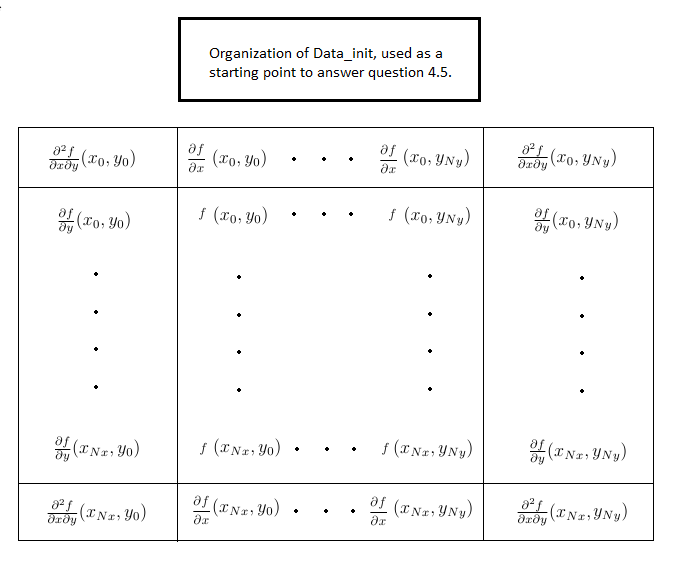
\includegraphics[scale=0.75]{q4_5.png}



\subsection{Question 4.6}


I will comment here the FORTRAN 90 / MPI code 
that is named "spline.f90", which answers this question (see folder question4\_6).\\

Some pictures are here to explain the mapping and the communications (\textit{spline1.png} and \textit{spline2.png}).\\

The general look of the code can obviously be improved by declaring constants and storing various aspect of the code in more files. The goal here was to provide something clear, that works.\\

Here, I provide a step-by-step explanation of what the code does :


\subsubsection{Running the program}


Parameters such as $P_x,P_y,N_x,N_y,x_{min},x_{max},y_{min},y_{max}$ are defined inside the spline.f90 file.\\

Once the number of processes in the x and y directions ($P_x,P_y$) have been set properly, the program \textbf{must} be executed with $P_x \times P_y$ processes.\\

If the user defined $P_x$ as 3 and $P_y$ as 5, then an example of correct calling instruction would be "\textit{mpiexec -machinefile hosts -n 15 ./spline}".


\subsubsection{Definitions}


We defined a simple function $f$ that we will only use to:\\
- Generate basic values on the sub-domain of each process.\\
- Check the results of the computations.\\

This function is initially set as $f(x,y)=x^2 +y^2$ and can be changed by the user.\\\\

We also defined a function $w$, which will be used to generate the $w_j$ coefficients, as defined by (4.13) on the problem statement.


\subsubsection{Assigning sub-domain, storing initial values}


As $P_x$ and $P_y$ are known, we can assign each process (according to its rank) its own subdomain $\Omega^{(I,J)}$ of $\Omega$.\\
Each process first computes its own $ (I,J)$ coordinates (stored in $I_{proc}$ and $ J_{proc}$ variables).\\

Up to this point, each process knows on which $\Omega^{(I,J)}$ it is working on. We now need to define and store the values of $f$ on the mesh defined by $N_x$ and $N_y$.\\

$N_x$ and $N_y$ are known, and to store what will be called the "base data", we need a matrix of size $(N_x+1) \times (N_y+1)$ (called "F\_ mat" in the program).\\

However, considering the required computations for the derivatives, I decided to work with an enlarged matrix of size\\ $(N_x+1+22) \times (N_y+1+22)$.\\

Indeed, formulae to get approximated derivatives require 10 neighbouring values in both directions, and should be computed for coordinates just "outside" of the Base\_ data matrix : this enlarges my matrix by 22 in both directions.\\

The "base data" will be written in the inner part of the "F\_ mat" matrix, such that we have enough empty space to store 11 numbers on every "edge" of this matrix later (hence why we can see the coordinates of the storage start at (12,12) in the code).\\

(please refer to image "\textit{spline1.png}")\\

The "external" empty parts of this matrix will be filled later, to store other values that will be sent by adjacent processes.


\subsubsection{Neighbours}


Each process has to determine its neighbours: this will allow it to send / receive the right data to / from the right processes.\\

Here, we will make use of periodicity of function $f$ on domain $\Omega$, such that each process has 4 neighbours (we will refer to them as $up$, $down$, $left$ and $right$), even though a process might be "on the border" of $\Omega$.\\
Once it has been done, sending and receiving the values each process needs is now possible.\\


\subsubsection{Communications, computations }


Each process has to make two sendings along the x-direction (both of size $11 \times (N_y+1)$, one of them to "up" and the other
 one to "down").\\ Up to that point, it is now possible to compute the required values of $\frac{\partial f}{\partial x}$ for $(x_i,y_j)$ with $ i \in${ $-1, N_x+1$} and $j \in$ {$0,...,N_y$}. However we are currently unable to compute the last ones (which are "in the corners").\\
 
\textit{Please, take a look at picture "\textit{spline2.png}".}\\
 
Later, two other communications along the y-direction (to "left" and "right", both of size $(Nx +23) \times 11$), will send all the data we need to compute the remaining derivatives:\\

-$\frac{\partial f}{\partial y}$ for $(x_i,y_j)$ with $ j \in${ $-1, N_y+1$} and $i \in$ {$-1,...,N_x$}\\

-$\frac{\partial ^2 f}{\partial x \partial y}$ in the "corners", by making use of the first sending that has already happened (which allows the "diagonal processes" to send the required data for $\frac{\partial ^2 f}{\partial x \partial y}$ indirectly).\\

- The four remaining values of $\frac{\partial f}{\partial x}$ in the corners, that we couldn't compute earlier.\\


Every time, the data is stored in a receive buffer (with a name such as "left\_ recv", for example) and then written on the "external parts" of the F\_mat matrix. Once it's done, we can compute the remaining derivatives.\\

Derivatives are respectively stored in matrix Fx ($2 \times (Ny+3)$),\\ Fy ($ (Nx+3) \times 2$) and Fxy ($2 \times 2$). This is only for test purposes: in question 4.7, I will store this data according to the picture in question 4.5, in variable Data\_Init.\\

The fact that we have a redundancy in the data on the border;  as it's shared by two "adjacent" processes (due to the definition of\\ $\Omega^{(I,J)} = [x^{(I)}, x^{(I+1)}] \times [y^{(J)}, y^{(J+1)}] $); has been taken into account in the code.\\

The code itself can obviously be improved (buffers, vectorializations...) but we decided to keep it as simple and clear as possible.


\subsubsection{Tests}


Test instructions are also provided at the end of the program. Those tests show that the base data of F\_ mat, Fx,Fy and Fxy matrices are correct, and that the "neighbour" procedure works properly.\\

The initial parameters make it easy to check that everything went as planned.\\


If we take $\Omega = [0,3] \times [0,5]$, with Px = 3, Py = 5 \\and Nx = Ny = 10, and take $f(x,y) = x^2 + y^2$, and finally have a look at process 7 (as in picture "spline1.png") we are to see:\\

- Base values in (the "inner part" of) F\_ mat from $f(1,2)=5$ to $f(2,3)=13$\\

- As the derivative with regards to $x$ is $2x$ , matrix Fx will contain a line of approximations  of $2 \times 0.9 = 1.8 $ and another one of approximations of $2 \times 2.1 = 4.2 $\\

- Same idea with the derivatives in $y$ except the values are $3.8$ and $6.2$\\

- The approx of the second order derivatives are numbers close to 0.\\

- That neighbours are correct.


\subsection{Question 4.7}

Using questions 4.5 and 4.6, we can now answer question 4.7.

We used only 2 files to do that, and the compilation was not possible as we don't have ifort at home and libraries lapack95 / blas95
cannot be handled by gfortran (we weren't able to understand / use MUMPS in time either).\\

Those are the "interpolation" files.\\

If it was possible, we would have resorted to better solvers, but we sticked to the triangular ones as we only solve LU systems here.\\

First, procedure from question 4.6 computes the approximation of the derivatives where we want, and directly fills matrix "Data\_Init" (that we need to compute the $\eta_{i,j}$).\\
Matrices Fx, Fy, and Fxy are not used anymore, and F\_mat it has served its purpose.\\

Then, we compute the $\eta_{i,j}$ like we did in the code answering question 4.6.\\

Data\_init structure's will be exactly as described in question 4.5, however, as we decided to build the spline on a bigger interpolation area (as explained in part 4.3), Data\_unit will be a $(N_x+5) \times (N_y+5)$ matrix.\\

This changes all the sizes of the systems to solve, as well as the indexation of Data\_unit, but it doesn't change anything to the procedure itself.


\newpage


\section{Resolution of the Laplace equation}


\subsection{Question 5.1}


We want to solve $ - \Delta_x \phi = \rho $ (of unknown function $\phi$) resorting to a finite different method, with periodic boundary conditions.\\

As $\; - \Delta_x \phi = - \left( \frac{\partial^2\phi}{\partial x^2} + \frac{\partial^2\phi}{\partial y^2} \right)$ and  $\phi''(x)= \frac{\phi(x+\Delta x) - 2\,\phi(x) + \phi(x-\Delta x)}{\Delta x^2} + O(\Delta x^2) \;\;\; $, we have: 

$$ - \Delta_x \phi(x,y) \approx \frac{ -\phi (x+\Delta x,y) +2 \phi (x,y) - \phi (x-\Delta x,y)}{\Delta x^2} +  \frac{ -\phi (x,y+\Delta y) + 2 \phi (x,y) - \phi (x,y-\Delta y)}{\Delta y^2}$$

We will work on the following numerical scheme :


$$\boxed{\frac{ -u_{i+1,j} +2\,u_{i,j} - u_{i-1,j}}{\Delta x^2} +  \frac{ -u_{i,j+1} + 2\,u_{i,j} - u_{i,j-1}}{\Delta y^2} = \rho_{i,j}}$$

with $u_{i,j} \approx \phi( x_i,y_j)$ and $\rho_{i,j} = \rho(x_i,y_j)$.\\

The form of the Matrix $\mathbb{A}$ is described in the following image, taking $\mathbb{A}\in\mathbf{R}^{20\times 20}$ such as a matrix per blocks ($4\times 4$ blocks here, so each block is of size $5\times 5$).\\

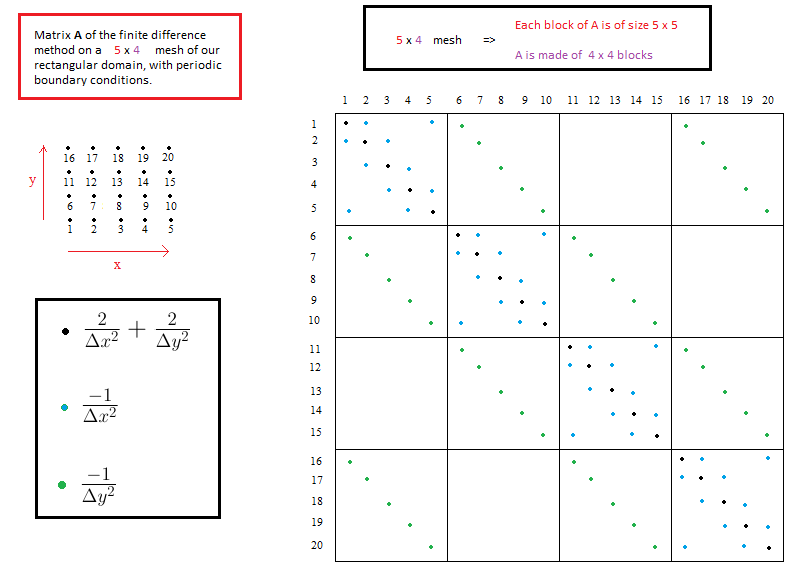
\includegraphics[scale=0.75]{Matrix_part5.png}

More generally if we consider $a = \frac{2}{\Delta x^2}+\frac{2}{\Delta y^2}$, $b = -\frac{1}{\Delta x^2}$, $c = -\frac{1}{\Delta y^2}$, $\mathbf{I}$ the identity matrix, $\mathbf{J} = c\,\mathbf{I}$ and :


$$
\mathbf{D} = \left(
\begin{array}{cccccccccc}
  a   &  b  &  0  &  \dots  &  \dots  &  \dots  &  0       &  b
      \\
b    &  a  &  b
  &  \ddots   &    &    &  \vdots  &   0    \\
 0   &  \ddots  &  \ddots  &  \ddots  &  \ddots  &    &  \vdots  & \vdots \\
  \vdots  &  \ddots  &  \ddots  &  \ddots  &  \ddots  &  \ddots  &  \vdots  & \vdots \\
  \vdots  &    &  \ddots  &  \ddots  &  \ddots  &  \ddots  &  0  & \vdots \\
  \vdots  &    &    &  \ddots  &  \ddots  &  \ddots  &  b  & 0 \\
  0  &    &    &    &  \ddots  &  \ddots  &  a  &  b    \\
  b  &  0  &  \dots  &  \dots  &  \dots  &  0  &  b       &  a
  
\end{array}
\right) 
$$ 

then we can write $\mathbb{A}$ with matrixes per blocks like this :
$$\mathbb{A} = \left(
\begin{array}{cccccccccc}
  \mathbf{D}   &  \mathbf{J}  &  \mathbf{0}  &  \dots  &  \dots  &  \dots  &  \mathbf{0}       &  \mathbf{J}
      \\
\mathbf{J}    &  \mathbf{D}  &  \mathbf{J}
  &  \ddots   &    &    &  \vdots  &   \mathbf{0}    \\
 \mathbf{0}   &  \ddots  &  \ddots  &  \ddots  &  \ddots  &    &  \vdots  & \vdots \\
  \vdots  &  \ddots  &  \ddots  &  \ddots  &  \ddots  &  \ddots  &  \vdots  & \vdots \\
  \vdots  &    &  \ddots  &  \ddots  &  \ddots  &  \ddots  &  \mathbf{0}  & \vdots \\
  \vdots  &    &    &  \ddots  &  \ddots  &  \ddots  &  \mathbf{J}  & \mathbf{0} \\
  \mathbf{0}  &    &    &    &  \ddots  &  \ddots  &  \mathbf{D}  &  \mathbf{J}    \\
  \mathbf{J}  &  \mathbf{0}  &  \dots  &  \dots  &  \dots  &  \mathbf{0}  &  \mathbf{J}       &  \mathbf{D}
\end{array}
\right) $$


We notice that, because of the periodic boundary conditions, we don't have to make any change to the right-hand side of equality $\;\; \mathbb{A} \cdot \bm{\phi} = \bm{\rho}$.\\

This means that to get the $u_{i,j}$, we will only have to build matrix $\mathbb{A}$ and vector $\\bm{rho}$, and then solve $\mathbb{A}\cdot \bm{\phi} = \bm{\rho}$.\\

This is what we do in the "Part5" FORTRAN 90 files.



\subsection{Question 5.2}


If we know $\phi$, we can use a second order accurate finite difference method to obtain $\textbf{E} = - \nabla_x \phi$ using : $ f'(x) = \frac {f (x + \Delta x) - f (x - \Delta x) }{2\, \Delta x} + O (\Delta x^2)$.
 
We can write, with $\Delta x$, $\Delta y > 0$ very small :

$$-\nabla_x \phi = \left(
\begin{array}{c c c}
      -\frac {\partial \phi (x,y)}{\partial x}\\
      -\frac {\partial \phi (x,y)}{\partial y}
 \end{array} \right) = \left(
\begin{array}{r c l}
      -\frac {\phi (x + \Delta x,y) - \phi (x - \Delta x,y) }{2\, \Delta x} + O (\Delta x^2)\\
      -\frac {\phi (x,y + \Delta y) - \phi (x,y - \Delta y) }{2\, \Delta y} + O (\Delta y^2)
 \end{array} \right) $$

Hence :

$$ \textbf{E} = \left(
\begin{array}{r c l}
      E_x\\
      E_y
 \end{array} \right) \approx \left(
\begin{array}{r c l}
      -\frac {\phi (x + \Delta x,y) - \phi (x - \Delta x,y) }{2 \Delta x}\\
      -\frac {\phi (x,y + \Delta y) - \phi (x,y - \Delta y) }{2 \Delta y}
 \end{array} \right) $$
 
We should keep the same $\Delta x$ and $\Delta y$ than previously.


\newpage

\section{Numerical results}


\subsection{Question 6.2}


\subsubsection{Notations and useful results}


We consider : \\
$
\begin{array}{l}
d\lambda = dx\,dy\,dv_x\,dv_y \; , \; k = \frac{N^0}{2\,\pi^{2}\,x_0\,y_0\,v_{x0}\,v_{y0}} , \; r = \frac{x^2}{x_0^2} + \frac{y^2}{y_0^2} 
 \mbox{ and } \;
I:\chi\mapsto\int_{\mathbb{R}_{+}}\int_0^{2\pi}\int_0^1\int_0^{2\pi} \chi^{2}\, e^{-\rho^{2}}\,r\,\rho\,d\theta\,dr\,d\phi\,d\rho \, .
\end{array}
$ \\

$f_p^0$ is a distribution so $I(\chi) < \infty$. \\
We will write $a = a(z)$ and $b = b(z)$ not forgetting that $a$ and $b$ depend on $z$. \\
We will use the constant $J$ defined in the question (2.4) :
$$ \boxed{J = \int_{0}^{2\pi}\cos(\theta)^2\,d\theta = \int_{0}^{2\pi}\sin(\theta)^2\,d\theta = \pi} $$
Let us  consider : $L = \int_{\mathbb{R}_+}\rho^{3}\,e^{-\rho^{2}}\,d\rho$.

\underline{Aim :} compute $I(\chi)$ for $\chi = 1, x, y, v_x, v_y$. \\

\subsubsection{Calculation of L}

Let us consider :$\alpha,\beta\in\mathbb{R}_{+}^{*}$ and
 $L_{\sqrt{\alpha}}^{\sqrt{\beta}} = \int_{\sqrt{\alpha}}^{\sqrt{\beta}}\rho^{3}\,e^{-\rho^{2}}\,d\rho$. \\
If we do the change of variable $\rho = \sqrt{x} \left(d\rho = \frac{dx}{2\sqrt{x}}\right)$, we have :
$$L_{\sqrt{\alpha}}^{\sqrt{\beta}} = \int_{\alpha}^{\beta} x\,\sqrt{x}\,e^{-x}\,\frac{dx}{2\sqrt{x}} = \frac{1}{2}\,\int_{\alpha}^{\beta} x\,e^{-x}\,dx $$
Now, we do an integration by parts using the functions $u,v\in C^1\left(\mathbb{R}_{+}\right)$ such that $u(x) = x$ and $v(x) = -e^{-x}$ : \\
$$L_{\sqrt{\alpha}}^{\sqrt{\beta}} = \frac{1}{2}\,\int_{\alpha}^{\beta} x\,e^{-x}\,dx = \frac{1}{2}\, \left[ -x\,e^{-x} \right]_a^b + \frac{1}{2}\,\int_{\alpha}^{\beta} e^{-x}\,dx  $$

Knowing that $\int_{0}^{\infty} e^{-\beta}\,d\beta < +\infty$ and $lim_{\beta \to \infty} \;\;\beta\,e^{-\beta} = 0$, we can write $L$ like this :
$$L = lim_{\beta \to + \infty} \left(lim_{\alpha \to 0} \;\;L_{\sqrt{\alpha}}^{\sqrt{\beta}} \right)
= lim_{\beta \to + \infty} \left(-\frac{\beta}{2}\,e^{-\beta} + \frac{1}{2}\,\int_{0}^{\beta} e^{-x}\,dx \right)
= 0 +\frac{1}{2}\,\int_{0}^{+\infty} e^{-x}\,dx = \frac{1}{2} \;\; \mbox{ so :}$$
$$\boxed{L = \frac{1}{2}}$$

\subsubsection{Changes of variable}

We will use the 2 following changes of variable :
$$
\boxed{\left\lbrace
    \begin{array}{ll}
x = x_0\,r\,\cos(\theta) \\
y = y_0\,r\,\sin(\theta)
    \end{array}
\right. 
\mbox{ and } \;\;\;
\left\lbrace
    \begin{array}{ll}
v_x = \sqrt{2}\,v_{x0}\,\rho\,\cos(\phi) \\
v_y = \sqrt{2}\,v_{y0}\,\rho\,\sin(\phi)
    \end{array}
\right.
}
$$

Obviously, their jacobians are respectively $x_0\,y_0\,r$ and $2\,v_{x0}\,v_{y0}\,\rho$ as we do polar changes of variables.

\subsubsection{Calculation of $\int_{\mathbb{R}^4} f_p^0\,d\lambda$}

Using the 2 previous changes of variable, we can compute $\int_{\mathbb{R}^4} f_p^0\,d\lambda$ :
\begin{align*}
\int_{\mathbb{R}^4} f_p^0\,d\lambda &= \int_{\mathbb{R}^2} \left(\int_{D} f_p^0\,dx\,dy \right)\,dv_x\,dv_y \;\; \mbox{ with } \; D = \left\lbrace (x,y)\in\mathbb{R}^2 \mbox{ such that } r^2\leq 1 \right\rbrace \\
&= \int_{\mathbb{R}^2} \left(\int_0^1\int_0^{2\pi} f_p^0\,x_0\,y_0\,r\,d\theta\,dr \right)\,dv_x\,dv_y \\
&= 2\,\pi\,x_0\,y_0\,\left(\int_0^1 r\,dr\right) \left(
\int_{\mathbb{R}^2} f_p^0\,dv_x\,dv_y\right) \\
&= \pi\,x_0\,y_0\,
\int_{\mathbb{R}^2} f_p^0\,dv_x\,dv_y \\
&= \pi\,x_0\,y_0\,
\int_{\mathbb{R}_{+}} \int_0^{2\pi} k\,e^{-\rho^{2}}\,2\,v_{x0}\,v_{y0}\,\rho\,d\phi\,d\rho \\
&= 4\pi^{2}\,x_0\,y_0\,v_{x0}\,v_{y0}\,k\,\left[ \frac{e^{-\rho^{2}}}{2} \right]_0^{+\infty} \\
&= 4\pi^{2}\,x_0\,y_0\,v_{x0}\,v_{y0}\,\frac{N^0}{2\,\pi^{2}\,x_0\,y_0\,v_{x0}\,v_{y0}}.\frac{1}{2} \\
&=N^0
\end{align*}
Hence : 
$$\boxed{\int_{\mathbb{R}^4} f_p^0(x,y,v_x,v_y)\,dx\,dy\,dv_x\,dv_y = N^0}$$

\subsubsection{Common calculation of $\chi_{RMS}(f_p^0)$}

\begin{align*}
\chi_{RMS}(f_p^0) &= \frac{ \int_{\mathbb{R}_{+}}\int_0^{2\pi}\int_0^1\int_0^{2\pi} \chi^{2}\, e^{-\rho^{2}}\,x_0\,y_0\,2\,vx_0\,vy_0\,r\,\rho\,d\theta\,dr\,d\phi\,d\rho}{\int_{\mathbb{R}_{+}}\int_0^{2\pi}\int_0^1\int_0^{2\pi} e^{-\rho^{2}}\,x_0\,y_0\,2\,vx_0\,vy_0\,r\,\rho\,d\theta\,dr\,d\phi\,d\rho} \\
&= \frac{ \int_{\mathbb{R}_{+}}\int_0^{2\pi}\int_0^1\int_0^{2\pi} \chi^{2}\, e^{-\rho^{2}}\,r\,\rho\,d\theta\,dr\,d\phi\,d\rho}{\int_{\mathbb{R}_{+}}\int_0^{2\pi}\int_0^1\int_0^{2\pi} e^{-\rho^{2}}\,r\,\rho\,d\theta\,dr\,d\phi\,d\rho} \\
&= \sqrt{\frac{I(\chi)}{I(1)}}
\end{align*}

Now, let us compute $I(\chi)$ for $\chi = 1,x,y,v_x,v_y$ :

\subsubsection{Calculation of $I(1)$}

\begin{align*}
I(1) &= 4\,\pi^{2} \left(\int_{0}^{1} r\,dr\right) \left(\int_{\mathbb{R}_{+}}\rho\,e^{-\rho^{2}}\,d\rho \right) \\
&= 4\,\pi^{2}.\frac{1}{2}.\frac{1}{2}
\end{align*}
Hence :
$$\boxed{I(1) = \pi^{2}}$$

\subsubsection{Calculation of $I(x)$, $I(y)$ and $x_{RMS}(f_p^0)$, $y_{RMS}(f_p^0)$}

\begin{align*}
I(x) &= \int_{\mathbb{R}_{+}}\int_0^{2\pi}\int_0^1\int_0^{2\pi} x_0^2\,r^3\rho\, e^{-\rho^{2}}\,\cos(\theta)^2\,d\theta\,dr\,d\phi\,d\rho \\
&= 2\,\pi\,x_0^2\,J\,\left(\int_{0}^{1} r^3\,dr\right) \left(\int_{\mathbb{R}_{+}}\rho\,e^{-\rho^{2}}\,d\rho \right) \\
&= 2\,x_0^2\,\pi^{2}.\frac{1}{4}.\frac{1}{2}
\end{align*}

Hence :
$$\boxed{I(x) = \frac{1}{4}\,x_0^2\,\pi^{2}}$$

We can compute $I(y)$ similarly, we get : 
$$\boxed{I(y) = \frac{1}{4}\,y_0^2\,\pi^{2}}$$

So we have : $x_{RMS}(f_p^0)^2 = \frac{1}{4}\,x_0^2 $. \\
Hence : 
$$\boxed{x_{RMS}(f_p^0) = \frac{x_0}{2}}$$
Similarly, we have : 
$$\boxed{y_{RMS}(f_p^0) = \frac{y_0}{2}}$$

\subsubsection{Calculation of $I(v_x)$, $I(v_y)$ and $v_{xRMS}(f_p^0)$, $v_{yRMS}(f_p^0)$}

\begin{align*}
I(v_x) &= \int_{\mathbb{R}_{+}}\int_0^{2\pi}\int_0^1\int_0^{2\pi} 2\,v_{x0}^2\,r\rho^3\, e^{-\rho^{2}}\,\cos(\phi)^2\,d\theta\,dr\,d\phi\,d\rho \\
&= 2\,v_{x0}^2\,(2\,\pi)\,\left(\int_{0}^{1} r\,dr\right)\,J\, \left(\int_{\mathbb{R}_{+}}\rho^{3}\,e^{-\rho^{2}}\,d\rho \right) \\
&= 2\,v_{x0}^2\,\pi^{2}\,L \\
&= v_{x0}^2\,\pi^{2}
\end{align*}

Hence :
$$\boxed{I(v_x) = v_{x0}^2\,\pi^{2}}$$

We can compute $I(v_y)$ similarly, we get : 
$$\boxed{I(v_y) = v_{y0}^2\,\pi^{2}}$$

So we have : $v_{xRMS}(f_p^0)^2 = v_{x0}^2 $. \\
Hence : 
$$\boxed{v_{xRMS}(f_p^0) = v_{x0}}$$
Similarly, we have : 
$$\boxed{v_{yRMS}(f_p^0) = v_{y0}}$$

\subsection{Question 6.3}

\subsubsection{Notations and useful results}

We consider : \\
$
\begin{array}{l}
d\lambda = dx\,dy\,dv_x\,dv_y \; , \; k = 4\,x_0\,y_0\,v_{x0}\,v_{y0} ,
 \mbox{ and } \;
I:\chi\mapsto\int_{\mathbb{R}^4} \chi^{2}\, \exp\left(-\frac{x^2}{2\,x_{0}^2}-\frac{y^2}{2\,y_{0}^2}-\frac{v_x^2}{2\,v_{x0}^2}-\frac{v_y^2}{2\,v_{y0}^2} \right) \,d\lambda \, .
\end{array}
$ \\

$f_p^0$ is a distribution so $I(\chi) < \infty$. \\

\subsubsection{Changes of variable}

We will use the 2 following changes of variable :
$$
\boxed{\left\lbrace
    \begin{array}{ll}
x = \sqrt{2}\,x_0\,r\,\cos(\theta) \\
y = \sqrt{2}\,y_0\,r\,\sin(\theta)
    \end{array}
\right. 
\mbox{ and } \;\;\;
\left\lbrace
    \begin{array}{ll}
v_x = \sqrt{2}\,v_{x0}\,\rho\,\cos(\phi) \\
v_y = \sqrt{2}\,v_{y0}\,\rho\,\sin(\phi)
    \end{array}
\right.
}
$$

Obviously, their jacobians are respectively $2\,x_0\,y_0\,r$ and $2\,v_{x0}\,v_{y0}\,\rho$ as we do polar changes of variables.

\subsubsection{Common calculation of $I(\chi)$}

\begin{align*}
I(\chi) &= \int_{\mathbb{R}^4} \chi^{2}\, \exp\left(-\frac{x^2}{2\,x_{0}^2}-\frac{y^2}{2\,y_{0}^2}-\frac{v_x^2}{2\,v_{x0}^2}-\frac{v_y^2}{2\,v_{y0}^2} \right) \,d\lambda \\
&= \int_{\mathbb{R}_{+}^2}\int_{[0,2\pi]^2} \chi^{2}\, e^{-(r^2+\rho^{2})}\,2\,x_0\,y_0\,2\,v_{x0}\,v_{y0}\,r\,\rho\,d\theta\,d\phi\,dr\,d\rho \\
&= k\, \int_{\mathbb{R}_{+}^2}\int_{[0,2\pi]^2} \chi^{2}\,r\,\rho\, e^{-(r^2+\rho^{2})}\,d\theta\,d\phi\,dr\,d\rho 
\end{align*}

\subsubsection{Calculation of $I(1)$}

\begin{align*}
I(1) &= 4\,\pi^{2}\,k \left(\int_{\mathbb{R}_{+}}r\,e^{-r^2}\,dr \right)^2 \\
&= 4\,\pi^{2}\,k\,\left(\frac{1}{2}\right)^2 \\
&= 4\,\pi^{2}\,x_0\,y_0\,2\,v_{x0}\,v_{y0}
\end{align*}
Hence :
$$\boxed{I(1) = = 4\,\pi^{2}\,x_0\,y_0\,2\,v_{x0}\,v_{y0}}$$

\subsubsection{Calculation of $\int_{\mathbb{R}^4}f_p^0\,d\lambda$}

$$\boxed{\int_{\mathbb{R}^4}f_p^0\,d\lambda = \frac{N^0}{4\,\pi^{2}\,x_0\,y_0\,2\,v_{x0}\,v_{y0}}\,I(1) = N^0}$$

\subsubsection{Calculation of $I(x)$ and $x_{RMS}(f_p^0)$}

\begin{align*}
I(x) &= \int_{\mathbb{R}_{+}^2}\int_{[0,2\pi]^2}  2\,x_0^2\,r^2\, e^{-r^2-\rho^{2}}\,\cos(\theta)^2\,r\,\rho\,d\theta\,d\phi\,dr\,d\rho \\
&= 2\,k\,x_0^2\,(2\pi)\,J\,\underbrace{\left(\int_{\mathbb{R}_{+}} r^3\,e^{-r^2}\,dr\right)}_{= 1/2} \underbrace{\left(\int_{\mathbb{R}_{+}}\rho\,e^{-\rho^{2}}\,d\rho \right)}_{= 1/2} \\
&= k\,x_0^2\,\pi^{2}
\end{align*}

So :
$${x_{RMS}(f_p^0)^2 = \frac{k\,x_0^2\,\pi^{2}}{k\,\pi^{2}}}$$
Hence :
$$\boxed{x_{RMS}(f_p^0) = x_0}$$

\subsubsection{Deduction of $y_{RMS}(f_p^0)$, $v_{xRMS}(f_p^0)$ and $v_{yRMS}(f_p^0)$}

The calculations are the same for $I(y)$, $I(v_x)$ and $I(v_y)$ so we can deduce that :
$$\boxed{y_{RMS}(f_p^0) = y_0}$$
$$\boxed{v_{xRMS}(f_p^0) = v_{x0}}$$
$$\boxed{v_{yRMS}(f_p^0) = v_{y0}}$$


\newpage

\section{Remarks}


\subsection{Concerning programs}


According to the compilator, sometimes program may work or not. I have no perticular problems in the computers of the room 106 but in my own PC, most of the programs which work good in the room 106 do not work on my PC. So, if there is a problem, for most of them (except the programs of the part 4 I just made this week-end), there is an executable which works. I do not know if the program I modify and complete this week are correct so I apologize if there are some errors into them.


\subsection{Concerning the questions 2.6. to 2.9.}


Reading the report, I understood functions $a$ and $b$ approximate functions $X$ and $Y$, so my idea was to remplace $X$ and $Y$ per $a$ and $b$ in the ODEs of the question 1.2. The hint given proposes us to use $\mathbf{E}^s_{KV}$ so I saw directly relations to the envelope equations appear, although I do not understand how can appear terms in $\cfrac{\epsilon_{x}^2}{a^3(z)}$ and $\cfrac{\epsilon_{y}^2}{b^3(z)}$. I think I have a part of the ideas we need to find these questions, hence I let my researches unless I know this is false, as it cames from the suppositions I made to do these questions.


\subsection{Concerning the tests}


I just do the test 1 with the FODO 2. It should not be difficult to implement the test 2 with some different things. Sometimes, I do not use what we should because we have to find it in another question and I do not have the time to put the data we could need to obtain exactly what we want.

\end{document}
